% Options for packages loaded elsewhere
\PassOptionsToPackage{unicode}{hyperref}
\PassOptionsToPackage{hyphens}{url}
%
\documentclass[
  man,floatsintext]{apa6}
\usepackage{amsmath,amssymb}
\usepackage{iftex}
\ifPDFTeX
  \usepackage[T1]{fontenc}
  \usepackage[utf8]{inputenc}
  \usepackage{textcomp} % provide euro and other symbols
\else % if luatex or xetex
  \usepackage{unicode-math} % this also loads fontspec
  \defaultfontfeatures{Scale=MatchLowercase}
  \defaultfontfeatures[\rmfamily]{Ligatures=TeX,Scale=1}
\fi
\usepackage{lmodern}
\ifPDFTeX\else
  % xetex/luatex font selection
\fi
% Use upquote if available, for straight quotes in verbatim environments
\IfFileExists{upquote.sty}{\usepackage{upquote}}{}
\IfFileExists{microtype.sty}{% use microtype if available
  \usepackage[]{microtype}
  \UseMicrotypeSet[protrusion]{basicmath} % disable protrusion for tt fonts
}{}
\makeatletter
\@ifundefined{KOMAClassName}{% if non-KOMA class
  \IfFileExists{parskip.sty}{%
    \usepackage{parskip}
  }{% else
    \setlength{\parindent}{0pt}
    \setlength{\parskip}{6pt plus 2pt minus 1pt}}
}{% if KOMA class
  \KOMAoptions{parskip=half}}
\makeatother
\usepackage{xcolor}
\usepackage{color}
\usepackage{fancyvrb}
\newcommand{\VerbBar}{|}
\newcommand{\VERB}{\Verb[commandchars=\\\{\}]}
\DefineVerbatimEnvironment{Highlighting}{Verbatim}{commandchars=\\\{\}}
% Add ',fontsize=\small' for more characters per line
\usepackage{framed}
\definecolor{shadecolor}{RGB}{248,248,248}
\newenvironment{Shaded}{\begin{snugshade}}{\end{snugshade}}
\newcommand{\AlertTok}[1]{\textcolor[rgb]{0.94,0.16,0.16}{#1}}
\newcommand{\AnnotationTok}[1]{\textcolor[rgb]{0.56,0.35,0.01}{\textbf{\textit{#1}}}}
\newcommand{\AttributeTok}[1]{\textcolor[rgb]{0.13,0.29,0.53}{#1}}
\newcommand{\BaseNTok}[1]{\textcolor[rgb]{0.00,0.00,0.81}{#1}}
\newcommand{\BuiltInTok}[1]{#1}
\newcommand{\CharTok}[1]{\textcolor[rgb]{0.31,0.60,0.02}{#1}}
\newcommand{\CommentTok}[1]{\textcolor[rgb]{0.56,0.35,0.01}{\textit{#1}}}
\newcommand{\CommentVarTok}[1]{\textcolor[rgb]{0.56,0.35,0.01}{\textbf{\textit{#1}}}}
\newcommand{\ConstantTok}[1]{\textcolor[rgb]{0.56,0.35,0.01}{#1}}
\newcommand{\ControlFlowTok}[1]{\textcolor[rgb]{0.13,0.29,0.53}{\textbf{#1}}}
\newcommand{\DataTypeTok}[1]{\textcolor[rgb]{0.13,0.29,0.53}{#1}}
\newcommand{\DecValTok}[1]{\textcolor[rgb]{0.00,0.00,0.81}{#1}}
\newcommand{\DocumentationTok}[1]{\textcolor[rgb]{0.56,0.35,0.01}{\textbf{\textit{#1}}}}
\newcommand{\ErrorTok}[1]{\textcolor[rgb]{0.64,0.00,0.00}{\textbf{#1}}}
\newcommand{\ExtensionTok}[1]{#1}
\newcommand{\FloatTok}[1]{\textcolor[rgb]{0.00,0.00,0.81}{#1}}
\newcommand{\FunctionTok}[1]{\textcolor[rgb]{0.13,0.29,0.53}{\textbf{#1}}}
\newcommand{\ImportTok}[1]{#1}
\newcommand{\InformationTok}[1]{\textcolor[rgb]{0.56,0.35,0.01}{\textbf{\textit{#1}}}}
\newcommand{\KeywordTok}[1]{\textcolor[rgb]{0.13,0.29,0.53}{\textbf{#1}}}
\newcommand{\NormalTok}[1]{#1}
\newcommand{\OperatorTok}[1]{\textcolor[rgb]{0.81,0.36,0.00}{\textbf{#1}}}
\newcommand{\OtherTok}[1]{\textcolor[rgb]{0.56,0.35,0.01}{#1}}
\newcommand{\PreprocessorTok}[1]{\textcolor[rgb]{0.56,0.35,0.01}{\textit{#1}}}
\newcommand{\RegionMarkerTok}[1]{#1}
\newcommand{\SpecialCharTok}[1]{\textcolor[rgb]{0.81,0.36,0.00}{\textbf{#1}}}
\newcommand{\SpecialStringTok}[1]{\textcolor[rgb]{0.31,0.60,0.02}{#1}}
\newcommand{\StringTok}[1]{\textcolor[rgb]{0.31,0.60,0.02}{#1}}
\newcommand{\VariableTok}[1]{\textcolor[rgb]{0.00,0.00,0.00}{#1}}
\newcommand{\VerbatimStringTok}[1]{\textcolor[rgb]{0.31,0.60,0.02}{#1}}
\newcommand{\WarningTok}[1]{\textcolor[rgb]{0.56,0.35,0.01}{\textbf{\textit{#1}}}}
\usepackage{graphicx}
\makeatletter
\def\maxwidth{\ifdim\Gin@nat@width>\linewidth\linewidth\else\Gin@nat@width\fi}
\def\maxheight{\ifdim\Gin@nat@height>\textheight\textheight\else\Gin@nat@height\fi}
\makeatother
% Scale images if necessary, so that they will not overflow the page
% margins by default, and it is still possible to overwrite the defaults
% using explicit options in \includegraphics[width, height, ...]{}
\setkeys{Gin}{width=\maxwidth,height=\maxheight,keepaspectratio}
% Set default figure placement to htbp
\makeatletter
\def\fps@figure{htbp}
\makeatother
\setlength{\emergencystretch}{3em} % prevent overfull lines
\providecommand{\tightlist}{%
  \setlength{\itemsep}{0pt}\setlength{\parskip}{0pt}}
\setcounter{secnumdepth}{-\maxdimen} % remove section numbering
% Make \paragraph and \subparagraph free-standing
\ifx\paragraph\undefined\else
  \let\oldparagraph\paragraph
  \renewcommand{\paragraph}[1]{\oldparagraph{#1}\mbox{}}
\fi
\ifx\subparagraph\undefined\else
  \let\oldsubparagraph\subparagraph
  \renewcommand{\subparagraph}[1]{\oldsubparagraph{#1}\mbox{}}
\fi
% definitions for citeproc citations
\NewDocumentCommand\citeproctext{}{}
\NewDocumentCommand\citeproc{mm}{%
  \begingroup\def\citeproctext{#2}\cite{#1}\endgroup}
\makeatletter
 % allow citations to break across lines
 \let\@cite@ofmt\@firstofone
 % avoid brackets around text for \cite:
 \def\@biblabel#1{}
 \def\@cite#1#2{{#1\if@tempswa , #2\fi}}
\makeatother
\newlength{\cslhangindent}
\setlength{\cslhangindent}{1.5em}
\newlength{\csllabelwidth}
\setlength{\csllabelwidth}{3em}
\newenvironment{CSLReferences}[2] % #1 hanging-indent, #2 entry-spacing
 {\begin{list}{}{%
  \setlength{\itemindent}{0pt}
  \setlength{\leftmargin}{0pt}
  \setlength{\parsep}{0pt}
  % turn on hanging indent if param 1 is 1
  \ifodd #1
   \setlength{\leftmargin}{\cslhangindent}
   \setlength{\itemindent}{-1\cslhangindent}
  \fi
  % set entry spacing
  \setlength{\itemsep}{#2\baselineskip}}}
 {\end{list}}
\usepackage{calc}
\newcommand{\CSLBlock}[1]{\hfill\break\parbox[t]{\linewidth}{\strut\ignorespaces#1\strut}}
\newcommand{\CSLLeftMargin}[1]{\parbox[t]{\csllabelwidth}{\strut#1\strut}}
\newcommand{\CSLRightInline}[1]{\parbox[t]{\linewidth - \csllabelwidth}{\strut#1\strut}}
\newcommand{\CSLIndent}[1]{\hspace{\cslhangindent}#1}
\ifLuaTeX
\usepackage[bidi=basic]{babel}
\else
\usepackage[bidi=default]{babel}
\fi
\babelprovide[main,import]{english}
% get rid of language-specific shorthands (see #6817):
\let\LanguageShortHands\languageshorthands
\def\languageshorthands#1{}
% Manuscript styling
\usepackage{upgreek}
\captionsetup{font=singlespacing,justification=justified}

% Table formatting
\usepackage{longtable}
\usepackage{lscape}
% \usepackage[counterclockwise]{rotating}   % Landscape page setup for large tables
\usepackage{multirow}		% Table styling
\usepackage{tabularx}		% Control Column width
\usepackage[flushleft]{threeparttable}	% Allows for three part tables with a specified notes section
\usepackage{threeparttablex}            % Lets threeparttable work with longtable

% Create new environments so endfloat can handle them
% \newenvironment{ltable}
%   {\begin{landscape}\centering\begin{threeparttable}}
%   {\end{threeparttable}\end{landscape}}
\newenvironment{lltable}{\begin{landscape}\centering\begin{ThreePartTable}}{\end{ThreePartTable}\end{landscape}}

% Enables adjusting longtable caption width to table width
% Solution found at http://golatex.de/longtable-mit-caption-so-breit-wie-die-tabelle-t15767.html
\makeatletter
\newcommand\LastLTentrywidth{1em}
\newlength\longtablewidth
\setlength{\longtablewidth}{1in}
\newcommand{\getlongtablewidth}{\begingroup \ifcsname LT@\roman{LT@tables}\endcsname \global\longtablewidth=0pt \renewcommand{\LT@entry}[2]{\global\advance\longtablewidth by ##2\relax\gdef\LastLTentrywidth{##2}}\@nameuse{LT@\roman{LT@tables}} \fi \endgroup}

% \setlength{\parindent}{0.5in}
% \setlength{\parskip}{0pt plus 0pt minus 0pt}

% Overwrite redefinition of paragraph and subparagraph by the default LaTeX template
% See https://github.com/crsh/papaja/issues/292
\makeatletter
\renewcommand{\paragraph}{\@startsection{paragraph}{4}{\parindent}%
  {0\baselineskip \@plus 0.2ex \@minus 0.2ex}%
  {-1em}%
  {\normalfont\normalsize\bfseries\itshape\typesectitle}}

\renewcommand{\subparagraph}[1]{\@startsection{subparagraph}{5}{1em}%
  {0\baselineskip \@plus 0.2ex \@minus 0.2ex}%
  {-\z@\relax}%
  {\normalfont\normalsize\itshape\hspace{\parindent}{#1}\textit{\addperi}}{\relax}}
\makeatother

\makeatletter
\usepackage{etoolbox}
\patchcmd{\maketitle}
  {\section{\normalfont\normalsize\abstractname}}
  {\section*{\normalfont\normalsize\abstractname}}
  {}{\typeout{Failed to patch abstract.}}
\patchcmd{\maketitle}
  {\section{\protect\normalfont{\@title}}}
  {\section*{\protect\normalfont{\@title}}}
  {}{\typeout{Failed to patch title.}}
\makeatother

\usepackage{xpatch}
\makeatletter
\xapptocmd\appendix
  {\xapptocmd\section
    {\addcontentsline{toc}{section}{\appendixname\ifoneappendix\else~\theappendix\fi\\: #1}}
    {}{\InnerPatchFailed}%
  }
{}{\PatchFailed}
\keywords{response times, event history analysis, Bayesian multi-level regression models, experimental psychology, cognitive psychology\newline\indent Word count: X}
\usepackage{lineno}

\linenumbers
\usepackage{csquotes}
\raggedbottom
\ifLuaTeX
  \usepackage{selnolig}  % disable illegal ligatures
\fi
\usepackage{bookmark}
\IfFileExists{xurl.sty}{\usepackage{xurl}}{} % add URL line breaks if available
\urlstyle{same}
\hypersetup{
  pdftitle={Event History Analyses for psychological time-to-event data: A tutorial in R with examples in Bayesian and frequentist workflows},
  pdfauthor={Sven Panis1 \& Richard Ramsey1},
  pdflang={en-EN},
  pdfkeywords={response times, event history analysis, Bayesian multi-level regression models, experimental psychology, cognitive psychology},
  hidelinks,
  pdfcreator={LaTeX via pandoc}}

\title{Event History Analyses for psychological time-to-event data: A tutorial in R with examples in Bayesian and frequentist workflows}
\author{Sven Panis\textsuperscript{1} \& Richard Ramsey\textsuperscript{1}}
\date{}


\shorttitle{A tutorial on hazard analysis}

\authornote{

Neural Control of Movement lab, Department of Health Sciences and Technology (D-HEST).
Social Brain Sciences lab, Department of Humanities, Social and Political Sciences (D-GESS).

The authors made the following contributions. Sven Panis: Conceptualization, Writing - Original Draft Preparation, Writing - Review \& Editing; Richard Ramsey: Conceptualization, Writing - Review \& Editing, Supervision.

Correspondence concerning this article should be addressed to Sven Panis, ETH GLC, room G16.2, Gloriastrasse 37/39, 8006 Zürich. E-mail: \href{mailto:sven.panis@hest.ethz.ch}{\nolinkurl{sven.panis@hest.ethz.ch}}

}

\affiliation{\vspace{0.5cm}\textsuperscript{1} ETH Zürich}

\abstract{%
Time-to-event data such as response times, saccade latencies, and fixation durations form a cornerstone of experimental psychology, and have had a widerspread impact on our understanding of human cognition. However, the orthodox method for analysing such data -- comparing means between conditions -- is known to conceal valuable information about the timeline of psychological effects, such as their onset time and duration. The ability to reveal finer-grained, ``temporal states'' of cognitive processes can have important consequences for theory development by qualitatively changing the key inferences that are drawn from psychological data. Moreover, well-established analytical approaches, such as event history analysis, are able to evaluate the detailed shape of time-to-event distributions, and thus characterise the timeline of psychological states. One barrier to wider use of event history analysis, however, is that the analytical workflow is typically more time-consuming and complex than orthodox approaches. To help achieve broader uptake, in this paper we outline a set of tutorials that detail how to implement one distributional method known as discrete-time event history analysis. We illustrate how to wrangle raw data files and calculate descriptive statistics, as well as how to calculate inferntial statistics via Bayesian and frequentist multi-level regression modelling. We touch upon several key aspects of the workflow, such as how to specify regression models, the implications for experimental design, as well as how to manage inter-individual differences. We finish the article by considering the benefits of the approach for understanding psychological states, as well as the limitations and future durections of this work. Finally, the project is written in R and freely available, which means the general approach can easily be adapted to other data sets, and all of the tutorials are avilable as .html files to widen access beyond R-users.
}



\begin{document}
\maketitle

\section{1. Introduction}\label{introduction}

\subsection{1.1 Motivation and background context: Comparing means versus distributional shapes}\label{motivation-and-background-context-comparing-means-versus-distributional-shapes}

In experimental psychology, it is standard practice to analyse response times (RTs), saccade latencies, and fixation durations by calculating average performance across a series of trials. Such mean-average comparisons have been the workhorse of experimental psychology over the last century, and have had a substantial impact of theory development and our understanding of the structure of cognition and brain function. However, differences in mean RT conceal when an experimental effect starts, how long it lasts, how it evolves with increasing waiting time, and whether its onset is time-locked to other events (insert REF). Such information is useful not only for interpretation of the effects, but also for cognitive psychophysiology and computational model selection (Panis, Schmidt, Wolkersdorfer, \& Schmidt, 2020).

As a simple illustration, Figure 1 shows the results of several simulated RT datasets, which show how mean-average comparisons between two conditions can conceal the shape of the underlying RT distributions. For instance, in examples 1-3, mean RT is always comparable between two conditions, while the distribution differs (Figure 1, top row). In contrast, in examples 4-6, mean RT is lower in condition 2 compared to condition 1, but the RT distribution differs in each case (Figure 1, bottom row). Therefore, a comparison of means would lead to a similar conclusion in examples 1-3, as well as examples 4-6, whereas a comparison of the distribution would lead to a different conclusion in every case.



\begin{figure}[H]

{\centering \includegraphics[width=0.9\linewidth,height=0.67\textheight,]{../sims/figures/haz_inset_facet} 

}

\caption{Means versus distributional shapes for six different simulated dataset examples. For our purposes here, it is enough to know that the distributions plotted represent the probability of an event occurring in that timebin, given that it has not yet occurred. Insets show mean reaction time per condition.}\label{fig:plot1}
\end{figure}

Why does this matter for research in psychology? Compared to the aggregation of data across trials, a distributional approach offers the possibility to reveal the timecourse of psychological states. As such, the approach permits different kinds of questions to be asked, different inferences to be made, and it holds the potential to discriminate between different theoretical accounts of psychological and/or brain-based processes.
For example, the distributions in Example 4 show that the effect starts around 200 ms and is gone by 600 ms. In contrast, in Example 5, the effect starts around 400 ms and is gone by 800 ms. And in the Example 6, the effect reverses around between 500 and 600 ms. What kind of theory or set of theories could account for such effects? Are there new auxiliary assumptions that theories need to adopt? And are there new experiments that need to be run to test the novel predictions that follow from these analyses? As we show later using concrete examples from past experimental data, for many psychological questions this ``temporal states'' information can be theoretically meaningful by leading to more fine-grained understanding of psychological processes as well as adding a relatively under-used dimension to our theory building toolkit.

From a historical perspective, it is worth noting that the development of analytical tools that can estimate or predict when events will occur is not a new endeavour.
Indeed, hundreds of years ago, analytical methods were developed to predict time to death (REFs).
The same logic has been applied to psychological time-to-event data, as previously demonstrated (Panis et al., 2020).
Here, in the paper, we hope to show the value of EHA for knowledge and theory building in cognitive psychology and related areas of research, such as cognitive neuroscience, as well as provide practical tutorials that provide step-by-step code and instructions in the hope that we can enable others to use EHA in a more routine, efficient and effective manner.

\subsection{1.2 Aims and structure of the paper}\label{aims-and-structure-of-the-paper}

In this paper, we focus on a distributional method known as discrete-time event history analysis, a.k.a. hazard analysis, duration analysis, failure-time analysis, survival analysis, and transition analysis.
We first provide a brief overview of hazard analysis to orient the reader to the basic concepts that we will use throughout the paper. However, this will remain relatively short, as this has been covered in detail before Singer and Willett (2003), Allison (1982), and Allison (2010), and our primary aim here is to introduce a set of tutorials, which explain \textbf{how} to do such analyses, rather than repeat in any detail \textbf{why} you should do them.

We then provide four different tutorials, each of which is written in the R programming language and publicly available on our Github and the Open Science Framework (OSF) pages, along with all of the other code and material associated with the project. The tutorials provide hands-on, concrete examples of key parts of the analytical process, so that others can apply the analyses to their own time-to-event data sets. Each tutorial is provided as an RMarkdown file, so that others can download and adapt the code to fit their own purposes. Additionally, each tutorial is made available as .html file, so that it can be viewed by any web browser, and thus available to those that do not use R.

In Tutorial 1, we illustrate how to process or ``wrangle'' a previously published RT dataset to calculate descriptive statistics when there is one independent variable. The descriptive statistics are plotted, and we comment on their interpretation. In Tutorial 2, we illustrate how one can fit Bayesian multi-level regression hazard models to the data using the R package brms. We discuss possible link functions, and plot the model-based effects of our predictors of interest. In Tutorial 3, we illustrate how to fit the same type of regression hazard models in a frequentist framework using the R package lme4. We then briefly compare and contrast these inferential frameworks when applied to EHA. In Tutorial 4, we provide a generalisation of the approach to illustrate one might descriptive statistics when using a more complex design, such as when there are two independent variables.

In summary, even though event history analyses is a widely used statistical tool and there already exist many excellent reviews (REFs) and tutorials (Allison, 2010) on its general use-cases, we are not aware of any tutorials that are aimed at psychological time-to-event data, and which provide worked examples of the key data processing and multi-level regression modelling steps.
Thereofore, our ultimate goal is twofold: first, we want to convince readers of the many benefits of using hazard analysis when dealing with time-to-event data with a focus on psychological time-to-event data, and second, we want to provide a set of practical tutorials, which provide step-by-step instructions on how you actually perform hazard analysis.

\section{2. A brief introduction to hazard analysis}\label{a-brief-introduction-to-hazard-analysis}

For a comprehensive background context to hazard analysis, we recommend several excellent textbooks (Singer \& Willett, 2003). Likewise, for general introduction to understanding regression equations, we recommend several introductory level textbooks (REFs). Our focus here is not on providing a detailed account of the underlying regression equations, since this topics has been comprehensively covered many times before. Instead, we want to provide an intuition to how EHA works in general as well as in the context of experimental psychology. As such, we only supply regression equations in supplementary materials and then refer to them in the text whenever relevant.

\subsection{2.1 Basic features of hazard analysis}\label{basic-features-of-hazard-analysis}

To apply event history analysis (EHA), one must be able to:

\begin{enumerate}
\def\labelenumi{\arabic{enumi}.}
\item
  define an event of interest that represents a qualitative change that can be situated in time (e.g., a button press, a saccade onset, a fixation offset, etc.)
\item
  define time point zero (e.g., target stimulus onset, fixation onset)
\item
  measure the passage of time between time point zero and event occurrence in discrete or continuous time units.
\end{enumerate}

The definition of hazard and the type of models employed depend on whether one is using continuous or discrete time units. Since our focus here is on hazard models that use discrete time units, we describe that approach. After dividing time in discrete, contiguous time bins indexed by t (e.g., t = 1:10 timebins), let RT be a discrete random variable denoting the rank of the time bin in which a particular person's response occurs in a particular experimental condition. For example, the first response could occur at 546 ms and it would be in timebin 6 (any RTs from 501 ms to 600). Continuous RT data is treated here as interval-censored data.

Discrete-time EHA focuses on the discrete-time hazard function and the discrete-time survivor function (Figure X). The equations that define both of these functions are reported in supplementary materials (part A). The discrete-time hazard probability gives you the probability that the event occurs (sometime) in bin t, given that the event does not occur in previous bins. In other words, it reflects the instantaneous likelihood that the event occurs in the current bin, given that it has not yet occurred in the past, i.e., in one of the prior bins. This conditionality in the definition of hazard is what makes the hazard function so diagnostic for studying event occurrence, as an event can physically not occur when it has already occurred before. In contrast, the discrete-time survivor function cumulates the bin-by-bin risks of event \emph{non}occurrence to obtain the probability that the event occurs after bin t. In other words, the survivor function reflects the likelihood that the event occurs in the future, i.e., in one of the subsequent timebins.

The survivor function can help to qualify or provide context to the interpretation of the hazard function. For example, it can give a sense of how many trials may contribute to that part of the distribution. If each participant completes 100 trials in an experiment, and the survivor function prob of 0.03, then only 3\% of trials remain beyond this point, which in this case would amount to 3 trials. Therefore, the error bars in this part of the distribution would be wider and less precise compared to other parts.



\begin{figure}[H]

{\centering 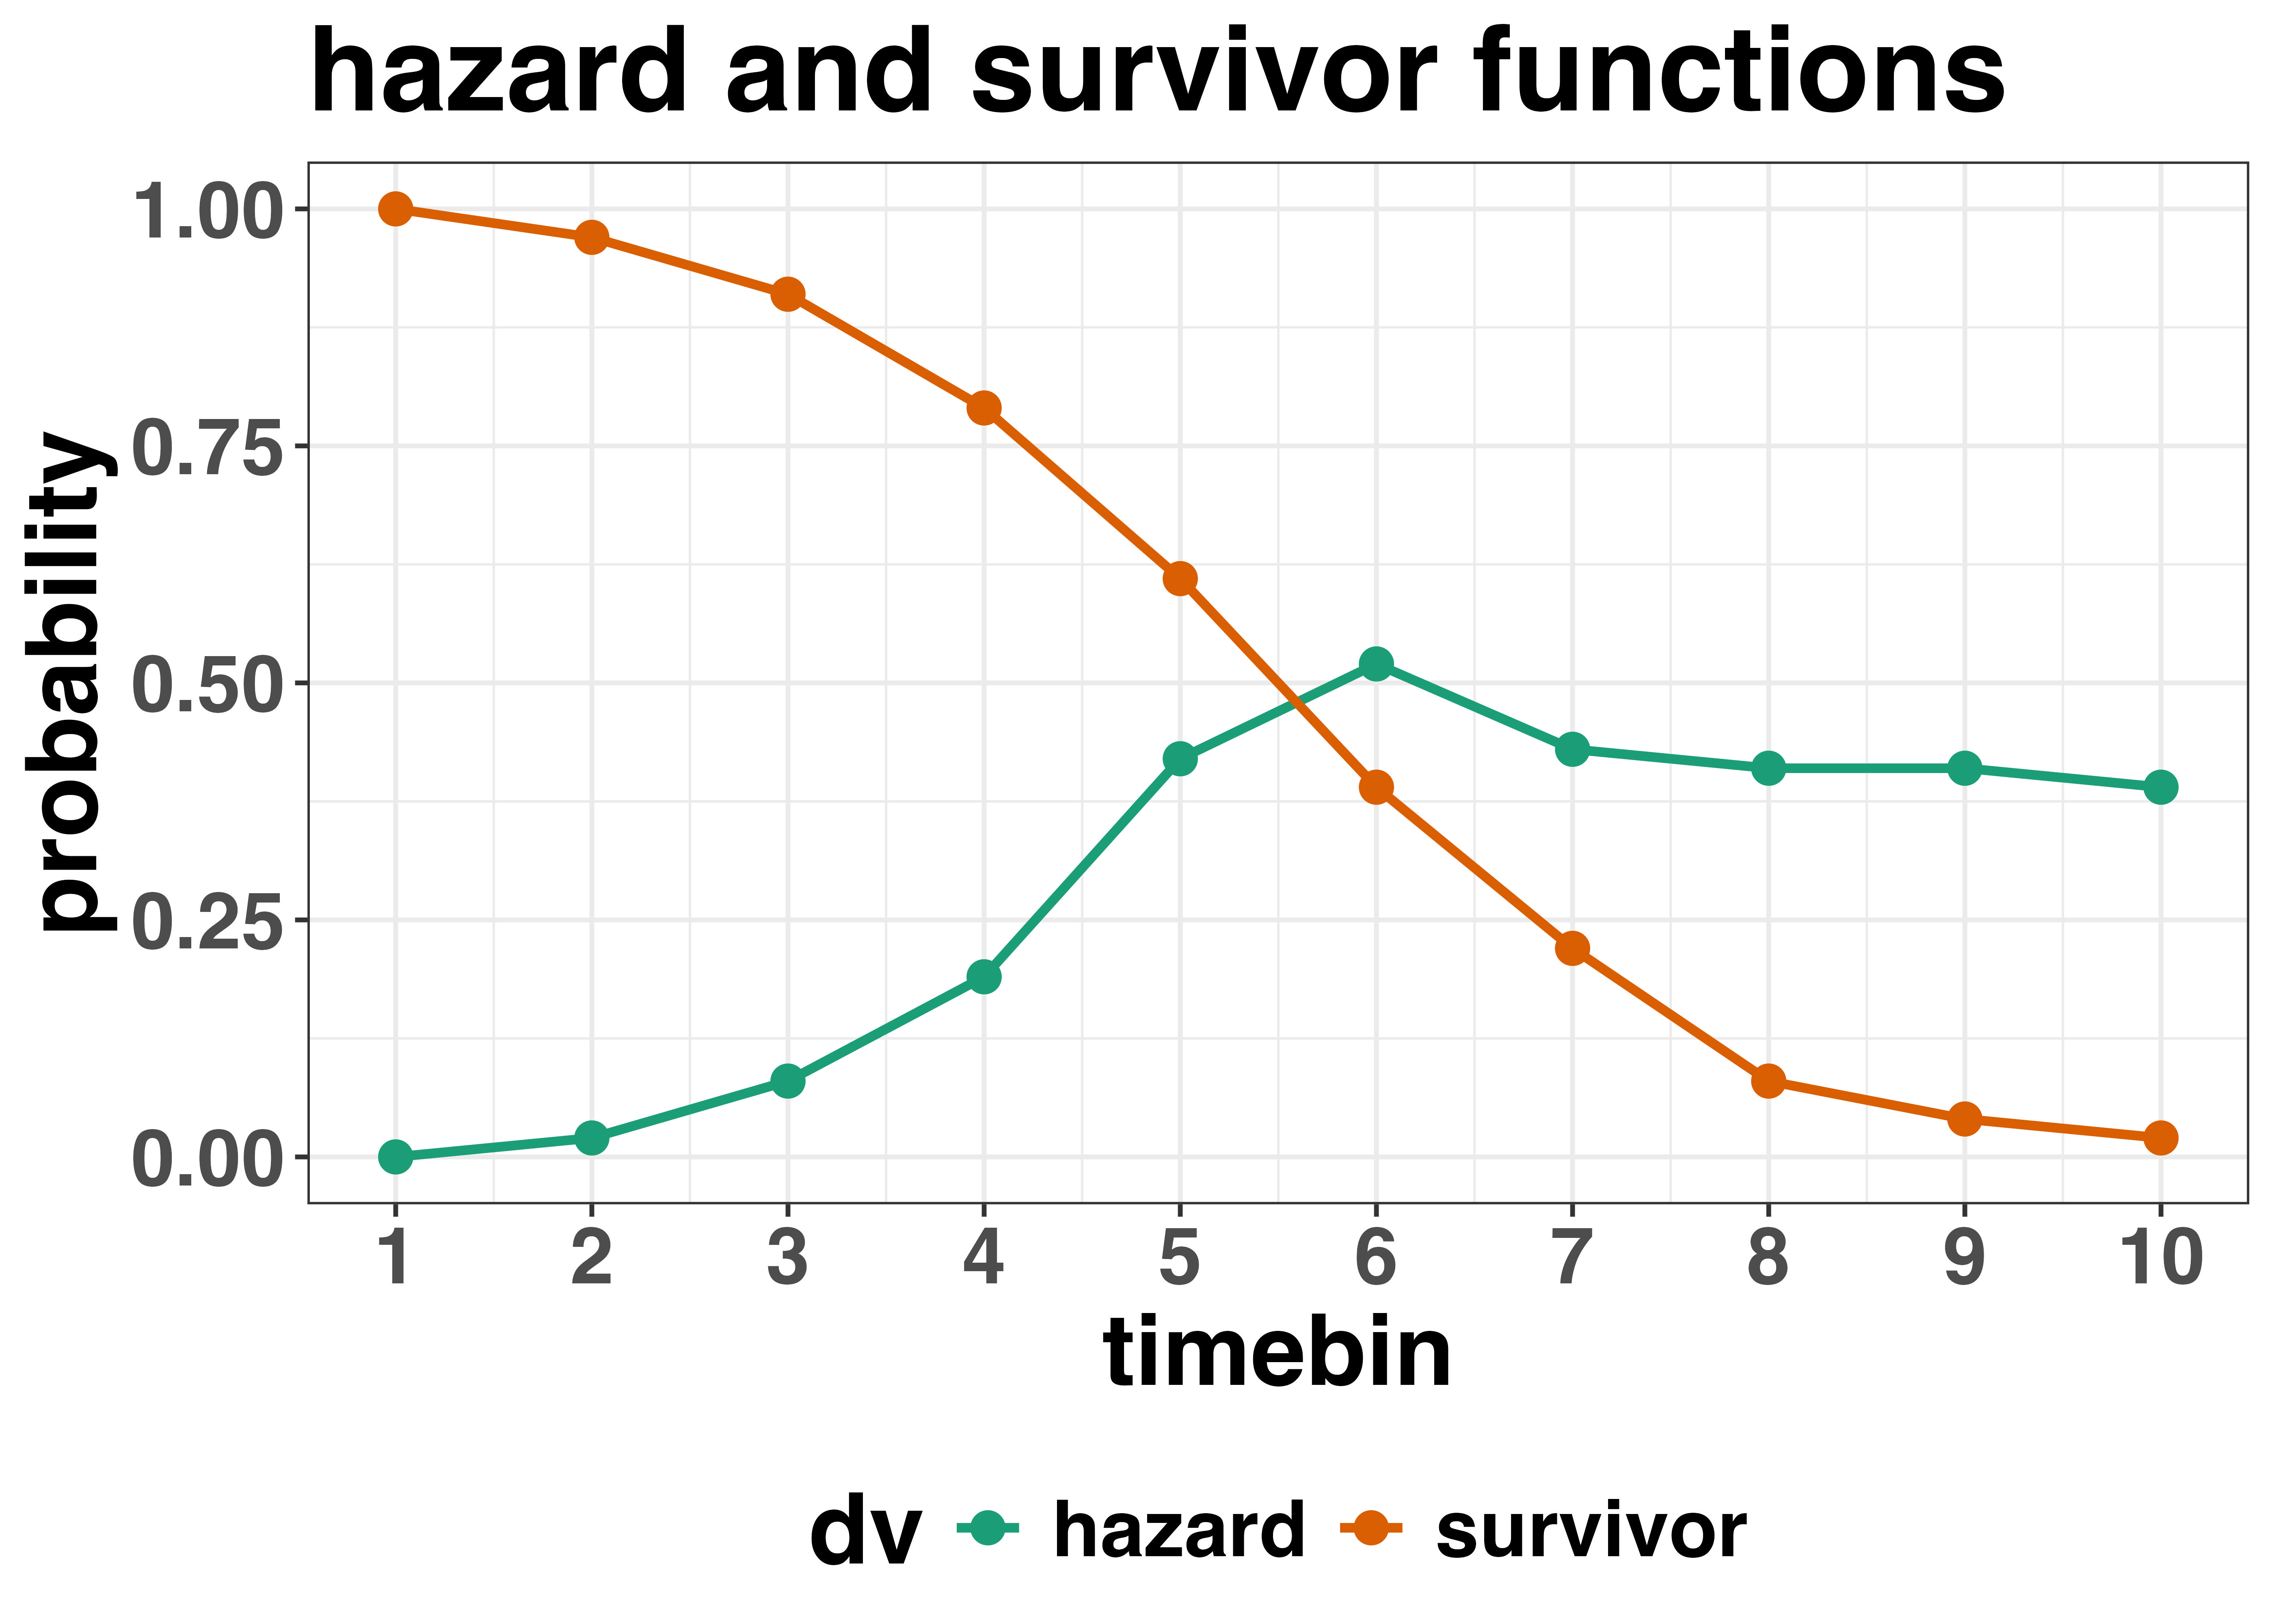
\includegraphics[width=0.8\linewidth,height=0.67\textheight,]{../sims/figures/haz_surv} 

}

\caption{Hazard and survivor functions}\label{fig:plot2-1}
\end{figure}

\subsection{2.2 Hazard analysis in the context of experimental psychology}\label{hazard-analysis-in-the-context-of-experimental-psychology}

\subsubsection{2.2.1 A worked example}\label{a-worked-example}

In the context of experimental psychology, it is common for participants to be presented with a task that has a right and a wrong answer. For example, a task may involve choosing between two response options with only one of them being correct. For such two-choice RT data, the discrete-time hazard function can be extended with the discrete-time conditional accuracy function (see equ. X in Supps), which gives you the probability that a response is correct given that it is emitted in time bin t (Allison, 2010; Kantowitz \& Pachella, 2021; Wickelgren, 1977).

Integrating results between hazard and conditional accuracy functions can be informative for understanding psychological processes. To illustrate, we consider a hypothetical example that is inspired by real data (Panis et al., 2016), but simplified to make the main point clearer (Figure 3). In a standard response priming paradigm, there is a prime stimulus (e.g., an arrow pointing left or right) followed by a target stimulus (another arrow pointing left or right). The prime can then be congruent or incongruent with the target. Figure 3 shows that the early upswing in hazard is equal for both conditions, and that early responses are always correct in .. and always incorrect in the incongruent condtion. Taken together, the results show that for early responses (\textless{} bin 6), responses always follow the prime (and not the target, as instructed). And then for later bins, response hazard is lower in incongruent compared to congruent trials, as \ldots..the prime can be overridden, as both conditions are now always correct. This is interesting because mean-average RT would only represent the overall ability of cognition to overcome interference, on average, across trials. And such a conclusion is not supported when the effects are explored over a timeline. Instead, the psychological conclusion is much more nuanced and suggests that multiple states start, stop and possibly interact over a particular temporal window.



\begin{figure}[H]

{\centering 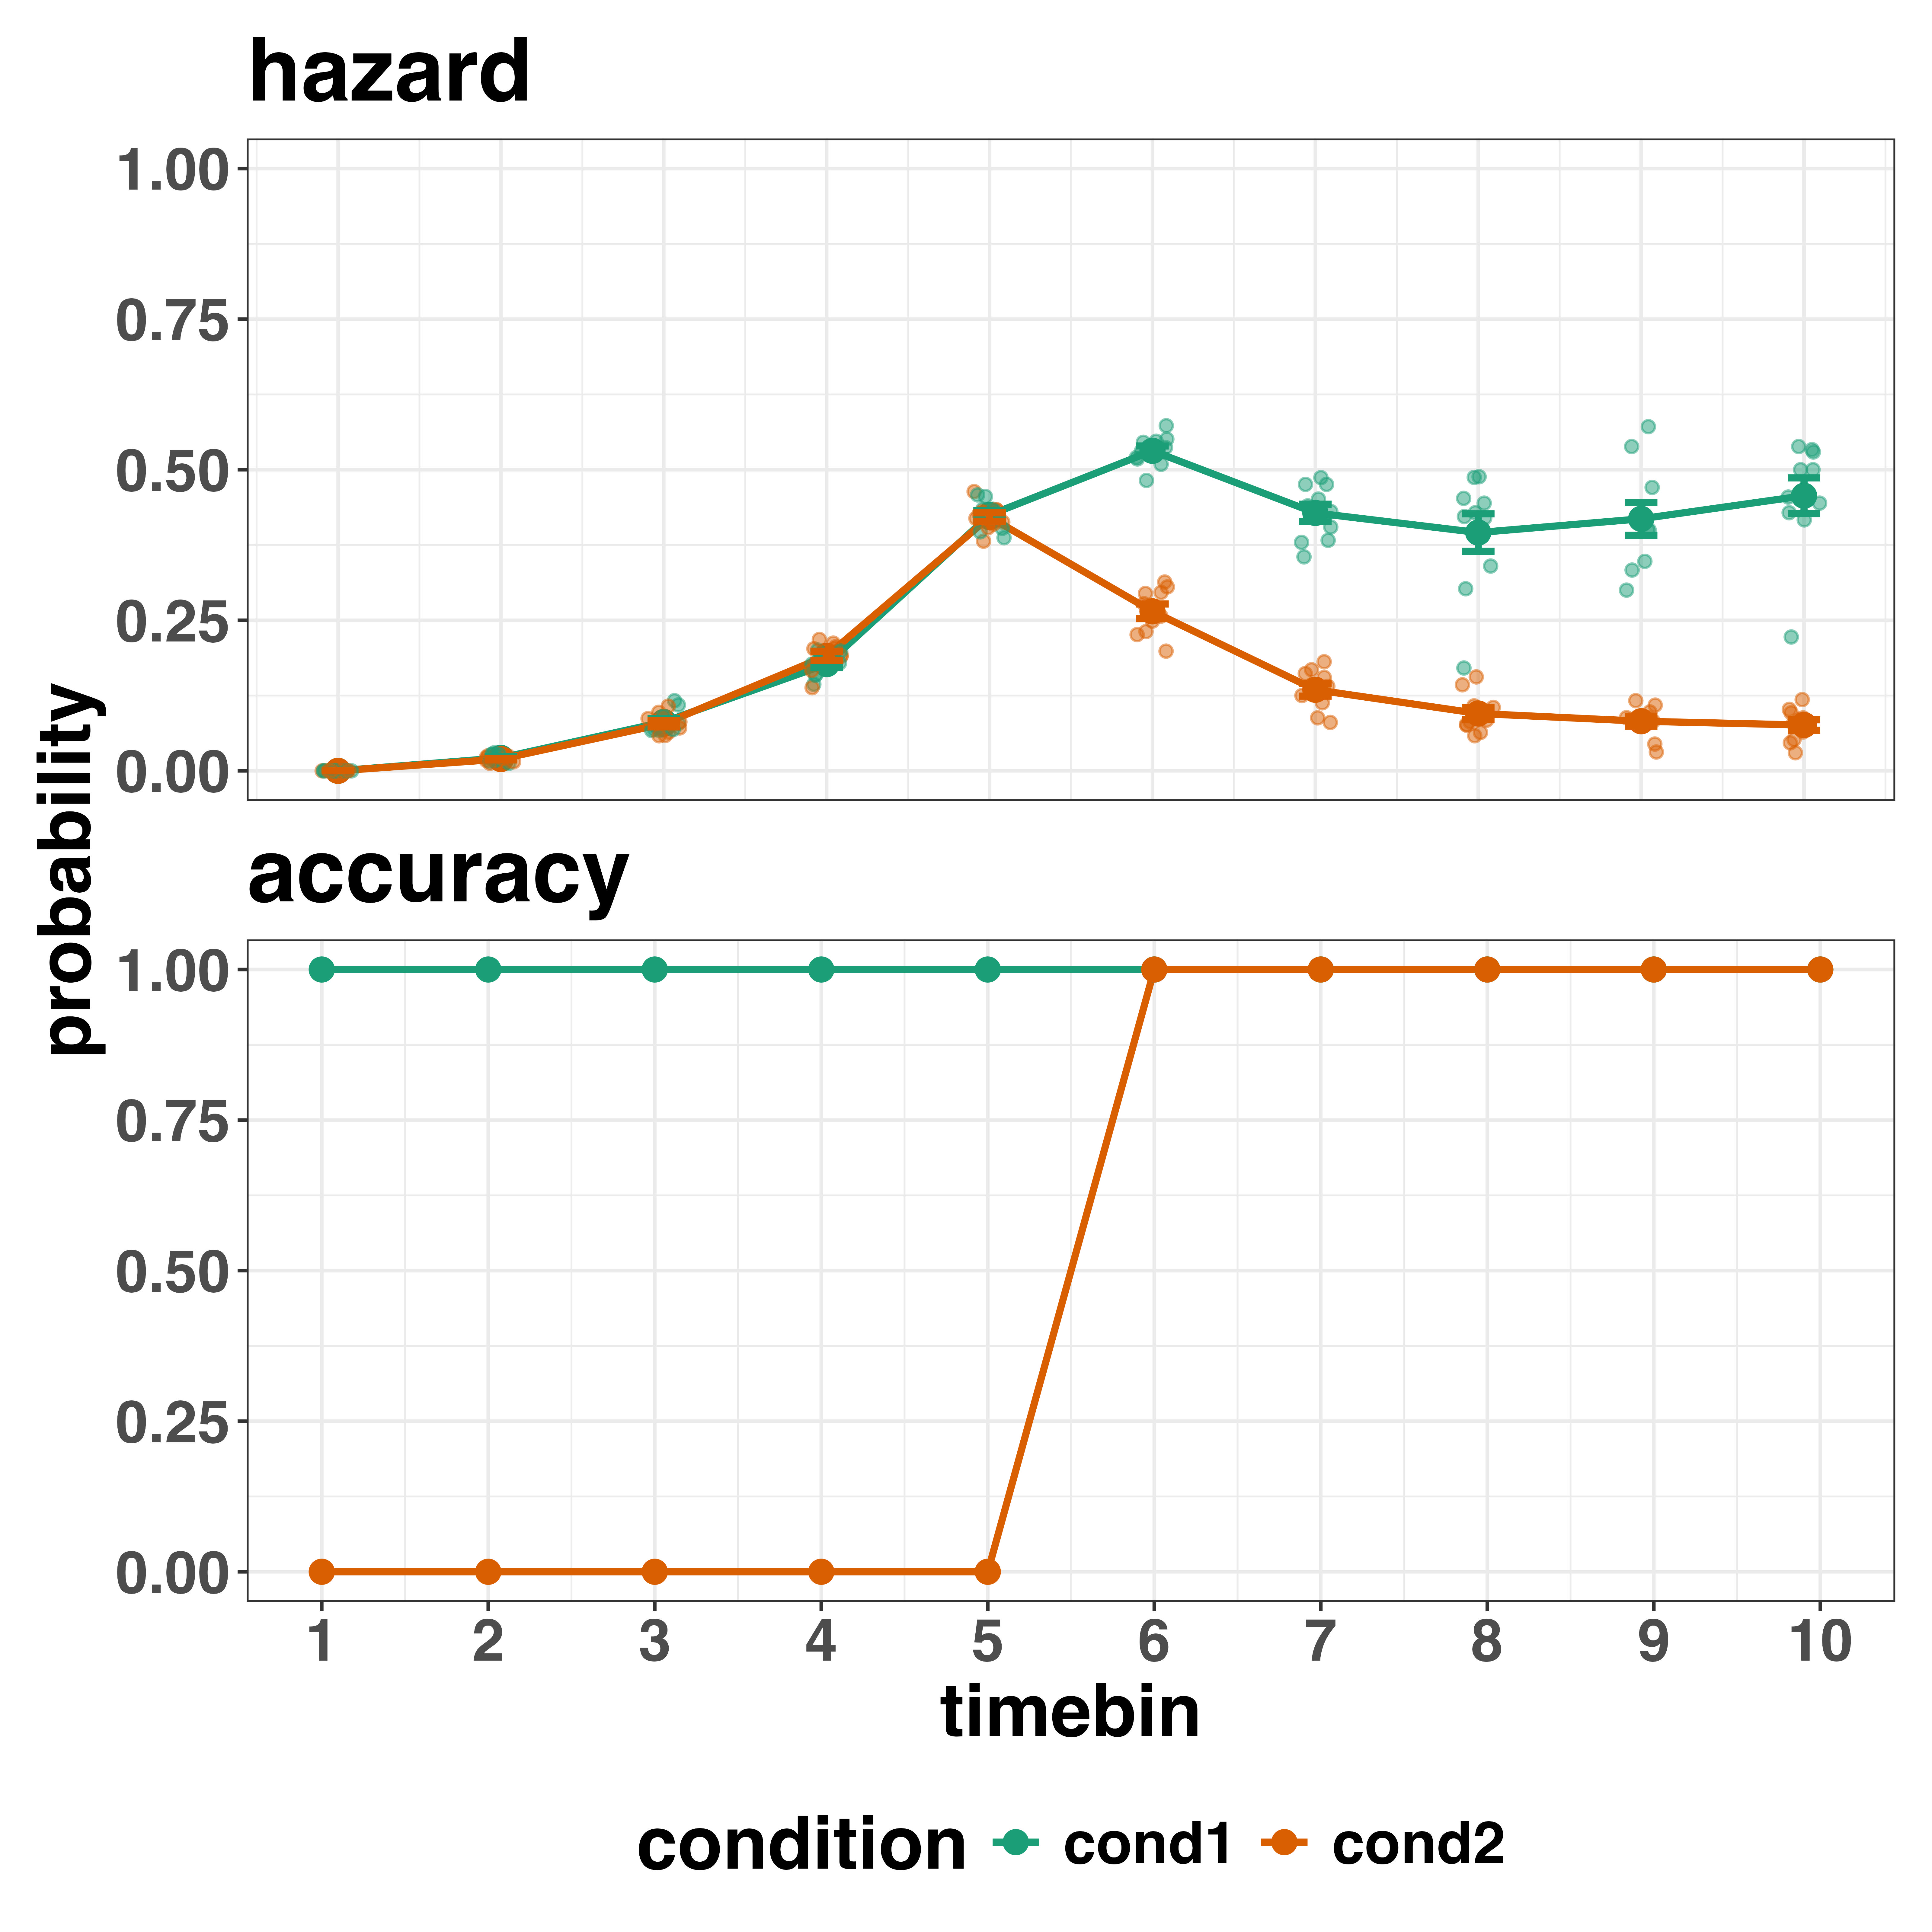
\includegraphics[width=0.8\linewidth,height=0.67\textheight,]{../sims/figures/haz_acc} 

}

\caption{Hazard and conditional accuracy}\label{fig:plot2-2}
\end{figure}

Unlocking the temporal states of cognitive processes can be revealing in and of itself for theory development and the understanding of basic psychological processes. Possibly more importantly, however, is that it simultaneously opens the door to address many new and previously unanswered questions. Do all participants show similar temporal states or are there individual differences? Do such individual differences extend to those individuals that have been diagnosed with some form of psychopathology? How do temporal states relate to brain-based mechanisms that might be studied using other methods from cognitive neuroscience? And how much of theory in cognitive psychology would be in need of revision if mean-average comparisons were supplemented with a temporal states approach?

\subsubsection{2.2.2 Implications for designing experiments}\label{implications-for-designing-experiments}

Performing hazard analyses in experimental psychology has implications for how experiments are designed. Indeed, if trials are categorised as a function of when they occur, then each timebin will only include a subset of the total number of trials. For example, let's consider an experiment where each participant performs 2 conditions and there are 100 trial repetitions per condition. Those 100 trials must be distributed in some manner across the chosen number of bins.

In such experimental designs, since the number of trials per condition are spread across bins, it is important to have a relatively large number of trial repetitions per participant and per condition. Accordingly, experiment designs using this approach typically focus on factorial, within-subject designs, in which a large number of observations are made on a relatively small number of participants (so-called small-\emph{N} designs). This approach emphasizes the precision and reproducibility of data patterns at the individual participant level to increase the inferential validity of the design (Baker et al., 2021; Smith \& Little, 2018).

In contrast to the large-\emph{N} design that typically average across many participants without being able to scrutinize individual data patterns, small-\emph{N} designs retain crucial information about the data patterns of individual observers. This can be advantageous whenever participants differ systematically in their strategies or in the time-courses of their effects, so that averaging them would lead to misleading data patterns. Note that because statistical power derives both from the number of participants and from the number of repeated measures per participant and condition, small-\emph{N} designs can still achieve what are generally considered acceptable levels of statistical power, if they have have a sufficient amount of data overall (Baker et al., 2021; Smith \& Little, 2018).

We used R (Version 4.4.0; R Core Team, 2024)\footnote{We, furthermore, used the R-packages \emph{bayesplot} (Version 1.11.1; Gabry, Simpson, Vehtari, Betancourt, \& Gelman, 2019), \emph{brms} (Version 2.21.0; Bürkner, 2017, 2018, 2021), \emph{citr} (Version 0.3.2; Aust, 2019), \emph{cmdstanr} (Version 0.8.1.9000; Gabry, Češnovar, Johnson, \& Bronder, 2024), \emph{dplyr} (Version 1.1.4; Wickham, François, Henry, Müller, \& Vaughan, 2023), \emph{forcats} (Version 1.0.0; Wickham, 2023a), \emph{ggplot2} (Version 3.5.1; Wickham, 2016), \emph{lme4} (Version 1.1.35.5; Bates, Mächler, Bolker, \& Walker, 2015), \emph{lubridate} (Version 1.9.3; Grolemund \& Wickham, 2011), \emph{Matrix} (Version 1.7.0; Bates, Maechler, \& Jagan, 2024), \emph{nlme} (Version 3.1.166; Pinheiro \& Bates, 2000), \emph{papaja} (Version 0.1.2.9000; Aust \& Barth, 2023), \emph{patchwork} (Version 1.2.0; Pedersen, 2024), \emph{purrr} (Version 1.0.2; Wickham \& Henry, 2023), \emph{RColorBrewer} (Version 1.1.3; Neuwirth, 2022), \emph{Rcpp} (Eddelbuettel \& Balamuta, 2018; Version 1.0.12; Eddelbuettel \& François, 2011), \emph{readr} (Version 2.1.5; Wickham, Hester, \& Bryan, 2024), \emph{RJ-2021-048} (Bengtsson, 2021), \emph{standist} (Version 0.0.0.9000; Girard, 2024), \emph{stringr} (Version 1.5.1; Wickham, 2023b), \emph{tibble} (Version 3.2.1; Müller \& Wickham, 2023), \emph{tidybayes} (Version 3.0.6; Kay, 2023), \emph{tidyr} (Version 1.3.1; Wickham, Vaughan, \& Girlich, 2024), \emph{tidyverse} (Version 2.0.0; Wickham et al., 2019), and \emph{tinylabels} (Version 0.2.4; Barth, 2023).} for all reported analyses. The content of the tutorials is mainly based on Allison (2010), Singer and Willett (2003), McElreath (2018), Kurz (2023a), and Kurz (2023b).

\section{3. An overview of the general analytical workflow}\label{an-overview-of-the-general-analytical-workflow}

Although the focus is on EHA, we also want to briefly comment on broader aspects of our general analytical workflow, which relate more to data science and data analysis workflows.

\subsection{3.1 Data science workflow and descriptive statistics}\label{data-science-workflow-and-descriptive-statistics}

Descriptive, data science workflow.
Data wrangling via tidyverse principles and a functional programming approach (cite R4DS textbook here).
Functional programming basically means you don't write your own loops but instead use functions that have been built and tested by others.
{[}{[}more here, as necessary{]}{]}.

\subsection{3.2 Inferential statistical approach}\label{inferential-statistical-approach}

Our lab adopts a estimation approach to multi-level regression (Kruschke \& Liddel, 2018; Winter, 2019), which is heavily influenced by Bayesian approach as suggested by Richard McElreath (McElreath, 2020; Kurz, 202?). We also use a ``keep it maximal'' approach to specifying varying (or random) effects (Barr et al., 2013). This means that wherever possible we include varying intercepts and slopes per participant
To make inferences, we use two main approaches. We compare models of different complexity, using information criteria, such as WAIC or LOO, to evaluate out-of-sample predictive accuracy. We also take the most complex model and evaluate key parameters of interest using point and interval estimates.

\section{4. Tutorials}\label{tutorials}

Tutorials 1a and 1b show how to calculate and plot the descriptive statistics when there are one and two independent variables, respectively. Tutorials 2a and 2b illustrate how to use Bayesian multilevel modeling to fit hazard and conditional accuracy models, respectively.
Tutorials 3a and 3b show how to implement, respectively, multilevel models for hazard and conditional accuracy in the frequentist framework.
Additionally, to further simplify the process for other users, the tutorials rely on a set of our own custom functions that make sub-processes easier to autmate, such as data wrangling and plotting functions.

Our list of tutorials is as follows:

1a. Wrangle raw data and descriptive stats for one independent variable.
1b. Wrangle raw data and descriptive stats for two independent variables.

2a. Bayesian multilevel modeling for h(t)
2b. Bayesian multilevel modeling for ca(t)

3a. Frequentist multilevel modeling for h(t)
3b. Frequentist multilevel modeling for ca(t)

Generalisation (T4). Should this be online in Supps?? It would make the main text shorter and simpler, but make it no less available. We could just have a sentence at the end of T1, which says that we provide a generalisation and extension in T4, which is in Supps.

Plannng (T5) - if we get a simulation and power analysis script working, which we are happy with then we could include it here.

\subsection{4.1 Tutorial 1a: Calculating descriptive statistics using a life table}\label{tutorial-1a-calculating-descriptive-statistics-using-a-life-table}

\subsubsection{4.1.1 Data wrangling aims}\label{data-wrangling-aims}

Our data wrangling procedures serve two related purposes. First, we want to summarise and visualise descriptive statistics that relate to our main research questions. Second, we want to produce two different datasets that can each be submitted to different types of inferential modelling approaches. The two types of data structure we label as `person-trial' data (Table 1) and `person-trial-bin' data (Table 2). The `person-trial' data will be familiar to most researchers who record behavioural responses from participants, as it represents the measured RT and accuracy per trial within an experiment. In contrast, the `person-trial-bin' data has a different, more extended structure, which indicates in which bin a response occurred, if at all, in each trial. Therefore, the `person-trial-bin' dataset generates a 0 in each bin until an event occurs and then it generates a 1 to signal an event has occurred. It is worth pointing out that there is no requirement for an event to occur at all (in any bin), as maybe there was no response on that trial or the event occurred after the timewindow of interest. Likewise, when the event occurs in bin 1 there would only be one row of data for that trial.





\begin{table}[H]

\begin{center}
\begin{threeparttable}

\caption{\label{tab:ca-data-table}Data structure for `person-trial' data}

\begin{tabular}{lllll}
\toprule
pid & \multicolumn{1}{c}{trial} & \multicolumn{1}{c}{condition} & \multicolumn{1}{c}{rt} & \multicolumn{1}{c}{accuracy}\\
\midrule
1 & 1 & congruent & 373.49 & 1\\
1 & 2 & incongruent & 431.31 & 1\\
1 & 3 & congruent & 455.43 & 0\\
1 & 4 & incongruent & 622.41 & 1\\
1 & 5 & incongruent & 535.98 & 1\\
1 & 6 & incongruent & 540.08 & 1\\
1 & 7 & congruent & 511.07 & 1\\
1 & 8 & incongruent & 444.42 & 1\\
1 & 9 & congruent & 678.69 & 1\\
1 & 10 & congruent & 549.79 & 1\\
\bottomrule
\addlinespace
\end{tabular}

\begin{tablenotes}[para]
\normalsize{\textit{Note.} The first 10 trials for participant 1 are shown. These data are simulated and for illustrative purposes only.}
\end{tablenotes}

\end{threeparttable}
\end{center}

\end{table}





\begin{table}[H]

\begin{center}
\begin{threeparttable}

\caption{\label{tab:ha-data-table}Data structure for `person-trial-bin' data}

\begin{tabular}{lllll}
\toprule
pid & \multicolumn{1}{c}{trial} & \multicolumn{1}{c}{condition} & \multicolumn{1}{c}{timebin} & \multicolumn{1}{c}{event}\\
\midrule
1 & 1 & congruent & 1 & 0\\
1 & 1 & congruent & 2 & 0\\
1 & 1 & congruent & 3 & 0\\
1 & 1 & congruent & 4 & 1\\
1 & 2 & incongruent & 1 & 0\\
1 & 2 & incongruent & 2 & 0\\
1 & 2 & incongruent & 3 & 0\\
1 & 2 & incongruent & 4 & 0\\
1 & 2 & incongruent & 5 & 1\\
\bottomrule
\addlinespace
\end{tabular}

\begin{tablenotes}[para]
\normalsize{\textit{Note.} The first 2 trials for participant 1 are shown. These data are simulated and for illustrative purposes only.}
\end{tablenotes}

\end{threeparttable}
\end{center}

\end{table}

\subsubsection{4.1.2 A real data wrangling example}\label{a-real-data-wrangling-example}

To illustrate how to quickly set up life tables for calculating the descriptive statistics (functions of discrete time), we use a published data set on masked response priming from Panis and Schmidt (2016).
In their first experiment, Panis and Schmidt (2016) presented a double arrow for 94 ms that pointed left or right as the target stimulus with an onset at time point zero in each trial. Participants had to indicate the direction in which the double arrow pointed using their corresponding index finger, within 800 ms after target onset. Response time and accuracy were recorded on each trial. Prime type (blank, congruent, incongruent) and mask type were manipulated. Here we focus on the subset of trials in which no mask was presented. The 13-ms prime stimulus was a double arrow with onset at -187 ms for the congruent (same direction as target) and incongruent (opposite direction as target) prime conditions.

There are several data wrangling steps to be taken. First, we need to load the data before we (a) supply required column names, and (b) specify the factor condition with the correct levels and labels.

The required column names are as follows:

\begin{itemize}
\tightlist
\item
  ``pid'', indicating unique participant IDs;
\item
  ``trial'', indicating each unique trial per participant;
\item
  ``condition'', a factor indicating the levels of the independent variable (1, 2, \ldots) and the corresponding labels;
\item
  ``rt'', indicating the response times in ms;
\item
  ``acc'', indicating the accuracies (1/0).
\end{itemize}

In the code of Tutorial 1a, this is accomplished as follows.

\scriptsize

\begin{Shaded}
\begin{Highlighting}[]
\NormalTok{data\_wr }\OtherTok{\textless{}{-}} \FunctionTok{read\_csv}\NormalTok{(}\StringTok{"../Tutorial\_1\_descriptive\_stats/data/DataExp1\_6subjects\_wrangled.csv"}\NormalTok{)}
\FunctionTok{colnames}\NormalTok{(data\_wr) }\OtherTok{\textless{}{-}} \FunctionTok{c}\NormalTok{(}\StringTok{"pid"}\NormalTok{,}\StringTok{"bl"}\NormalTok{,}\StringTok{"tr"}\NormalTok{,}\StringTok{"condition"}\NormalTok{,}\StringTok{"resp"}\NormalTok{,}\StringTok{"acc"}\NormalTok{,}\StringTok{"rt"}\NormalTok{,}\StringTok{"trial"}\NormalTok{) }
\NormalTok{data\_wr }\OtherTok{\textless{}{-}}\NormalTok{ data\_wr }\SpecialCharTok{\%\textgreater{}\%} 
  \FunctionTok{mutate}\NormalTok{(}\AttributeTok{condition =}\NormalTok{ condition }\SpecialCharTok{+} \DecValTok{1}\NormalTok{, }\CommentTok{\# original levels were 0, 1, 2.}
         \AttributeTok{condition =} \FunctionTok{factor}\NormalTok{(condition, }\AttributeTok{levels=}\FunctionTok{c}\NormalTok{(}\DecValTok{1}\NormalTok{,}\DecValTok{2}\NormalTok{,}\DecValTok{3}\NormalTok{), }\AttributeTok{labels=}\FunctionTok{c}\NormalTok{(}\StringTok{"blank"}\NormalTok{,}\StringTok{"congruent"}\NormalTok{,}\StringTok{"incongruent"}\NormalTok{)))}
\end{Highlighting}
\end{Shaded}

\normalsize

Next, we can set up the life tables and plots of the discrete-time functions h(t), S(t) and ca(t). To do so using a functional programming approach, one has to nest the data within participants using the group\_nest() function, and supply a user-defined censoring time and bin width to our function ``censor()'', as follows.

\scriptsize

\begin{Shaded}
\begin{Highlighting}[]
\NormalTok{data\_nested }\OtherTok{\textless{}{-}}\NormalTok{ data\_wr }\SpecialCharTok{\%\textgreater{}\%} \FunctionTok{group\_nest}\NormalTok{(pid)}
\NormalTok{data\_final }\OtherTok{\textless{}{-}}\NormalTok{ data\_nested }\SpecialCharTok{\%\textgreater{}\%} 
  \FunctionTok{mutate}\NormalTok{(}\AttributeTok{censored  =} \FunctionTok{map}\NormalTok{(data, censor, }\DecValTok{600}\NormalTok{, }\DecValTok{40}\NormalTok{)) }\SpecialCharTok{\%\textgreater{}\%}   \CommentTok{\# ! user input: censoring time, and bin width}
  \FunctionTok{mutate}\NormalTok{(}\AttributeTok{ptb\_data  =} \FunctionTok{map}\NormalTok{(censored, ptb)) }\SpecialCharTok{\%\textgreater{}\%}           \CommentTok{\# create person{-}trial{-}bin dataset}
  \FunctionTok{mutate}\NormalTok{(}\AttributeTok{lifetable =} \FunctionTok{map}\NormalTok{(ptb\_data, setup\_lt)) }\SpecialCharTok{\%\textgreater{}\%}      \CommentTok{\# create life tables without ca(t)}
  \FunctionTok{mutate}\NormalTok{(}\AttributeTok{condacc   =} \FunctionTok{map}\NormalTok{(censored, calc\_ca)) }\SpecialCharTok{\%\textgreater{}\%}       \CommentTok{\# calculate ca(t)}
  \FunctionTok{mutate}\NormalTok{(}\AttributeTok{lifetable\_ca =} \FunctionTok{map2}\NormalTok{(lifetable, condacc, join\_lt\_ca)) }\SpecialCharTok{\%\textgreater{}\%}    \CommentTok{\# create life tables with ca(t)}
  \FunctionTok{mutate}\NormalTok{(}\AttributeTok{plot      =} \FunctionTok{map2}\NormalTok{(}\AttributeTok{.x =}\NormalTok{ lifetable\_ca, }\AttributeTok{.y =}\NormalTok{ pid, plot\_eha,}\DecValTok{1}\NormalTok{))  }\CommentTok{\# create plots }
\end{Highlighting}
\end{Shaded}

\normalsize

Note that the censoring time should be a multiple of the bin width (both in ms). The censoring time should be a time point after which no informative responses are expected anymore. In experiments that implement a response deadline in each trial the censoring time can equal that deadline time point. Trials with a RT larger than the censoring time, or trials in which no response is emitted during the data collection period, are treated as right-censored observations in EHA. In other words, these trials are not discarded, because they contain the information that the event did not occur before the censoring time. Removing such trials before calculating the mean event time can introduce a sampling bias (REFs). The person-trial-bin oriented dataset has one row for each time bin of each trial that is at risk for event occurrence. The variable ``event'' in the person-trial-bin oriented data set indicates whether a response occurs (1) or not (0) for each bin.

The next step is to plot the data using our custom made plotting tool plot\_eha(). When creating the plots, some warning messages will likely be generated, like these:

\begin{itemize}
\tightlist
\item
  Removed 2 rows containing missing values or values outside the scale range (\texttt{geom\_line()}).
\item
  Removed 2 rows containing missing values or values outside the scale range (\texttt{geom\_point()}).
\item
  Removed 2 rows containing missing values or values outside the scale range (\texttt{geom\_segment()}).
\end{itemize}

The warning messages are generated because some bins have no hazard and ca(t) estimates, and no error bars. They can thus safely be ignored.
One can now inspect different aspects, including the life table for a particular condition of a particular subject, and a plot of the different functions for a particular participant. It is important to visually inspect the functions first for each participant, in order to identify possible cheaters (e.g., a flat conditional accuracy function at .5 indicates (s)he was only guessing), outlying individulas, and/or different groups with qualitatively different behavior.

Table 3 shows the life table for condition ``blank'' (no prime stimulus presented) for participant 6 - compare to Figure 1. A life table includes for each time bin, the risk set (number of trials that are event-free at the start of the bin), the number of observed events, and the estimates of h(t), S(t), possibly ca(t), and their estimated standard errors (se). At time point zero, no events can occur and therefore h(t) and ca(t) are undefined.

Figure 4 displays the discrete-time hazard, survivor, and conditional accuracy functions for each prime condition for participant 6. By using discrete-time h(t) functions of event occurrence - in combination with ca(t) functions for two-choice tasks - one can provide an unbiased, time-varying, and probabilistic description of the latency and accuracy of responses based on all trials of any data set.

For example, for participant 6, the estimated hazard values in bin (240,280{]} are 0.03, 0.17, and 0.20 for the blank, congruent, and incongruent prime conditions, respectively. In other words, when the waiting time has increased until \emph{240 ms} after target onset, then the conditional probability of response occurrence in the next 40 ms is more than five times larger for both prime-present conditions, compared to the blank prime condition.

Furthermore, the estimated conditional accuracy values in bin (240,280{]} are 0.29, 1, and 0 for the blank, congruent, and incongruent prime conditions, respectively. In other words, if a response is emitted in bin (240,280{]}, then the probability that it is correct is estimated to be 0.29, 1, and 0 for the blank, congruent, and incongruent prime conditions, respectively.





\begin{table}[H]

\begin{center}
\begin{threeparttable}

\caption{\label{tab:life-table}The life table for the blank prime condition of participant 6.}

\begin{tabular}{lllllllll}
\toprule
bin & \multicolumn{1}{c}{risk\_set} & \multicolumn{1}{c}{events} & \multicolumn{1}{c}{hazard} & \multicolumn{1}{c}{se\_haz} & \multicolumn{1}{c}{survival} & \multicolumn{1}{c}{se\_surv} & \multicolumn{1}{c}{ca} & \multicolumn{1}{c}{se\_ca}\\
\midrule
0.00 & 220.00 & NA & NA & NA & 1.00 & 0.00 & NA & NA\\
40.00 & 220.00 & 0.00 & 0.00 & 0.00 & 1.00 & 0.00 & NA & NA\\
80.00 & 220.00 & 0.00 & 0.00 & 0.00 & 1.00 & 0.00 & NA & NA\\
120.00 & 220.00 & 0.00 & 0.00 & 0.00 & 1.00 & 0.00 & NA & NA\\
160.00 & 220.00 & 0.00 & 0.00 & 0.00 & 1.00 & 0.00 & NA & NA\\
200.00 & 220.00 & 0.00 & 0.00 & 0.00 & 1.00 & 0.00 & NA & NA\\
240.00 & 220.00 & 0.00 & 0.00 & 0.00 & 1.00 & 0.00 & NA & NA\\
280.00 & 220.00 & 7.00 & 0.03 & 0.01 & 0.97 & 0.01 & 0.29 & 0.17\\
320.00 & 213.00 & 13.00 & 0.06 & 0.02 & 0.91 & 0.02 & 0.77 & 0.12\\
360.00 & 200.00 & 26.00 & 0.13 & 0.02 & 0.79 & 0.03 & 0.92 & 0.05\\
400.00 & 174.00 & 40.00 & 0.23 & 0.03 & 0.61 & 0.03 & 1.00 & 0.00\\
440.00 & 134.00 & 48.00 & 0.36 & 0.04 & 0.39 & 0.03 & 0.98 & 0.02\\
480.00 & 86.00 & 37.00 & 0.43 & 0.05 & 0.22 & 0.03 & 1.00 & 0.00\\
520.00 & 49.00 & 32.00 & 0.65 & 0.07 & 0.08 & 0.02 & 1.00 & 0.00\\
560.00 & 17.00 & 9.00 & 0.53 & 0.12 & 0.04 & 0.01 & 1.00 & 0.00\\
600.00 & 8.00 & 4.00 & 0.50 & 0.18 & 0.02 & 0.01 & 1.00 & 0.00\\
\bottomrule
\addlinespace
\end{tabular}

\begin{tablenotes}[para]
\normalsize{\textit{Note.} The column named ``bin'' indicates the endpoint of each time bin (in ms), and includes time point zero. For example the first bin is (0,40{]} with the starting point excluded and the endpoint included. se = standard error. ca = conditional accuracy.}
\end{tablenotes}

\end{threeparttable}
\end{center}

\end{table}



\begin{figure}[H]

{\centering 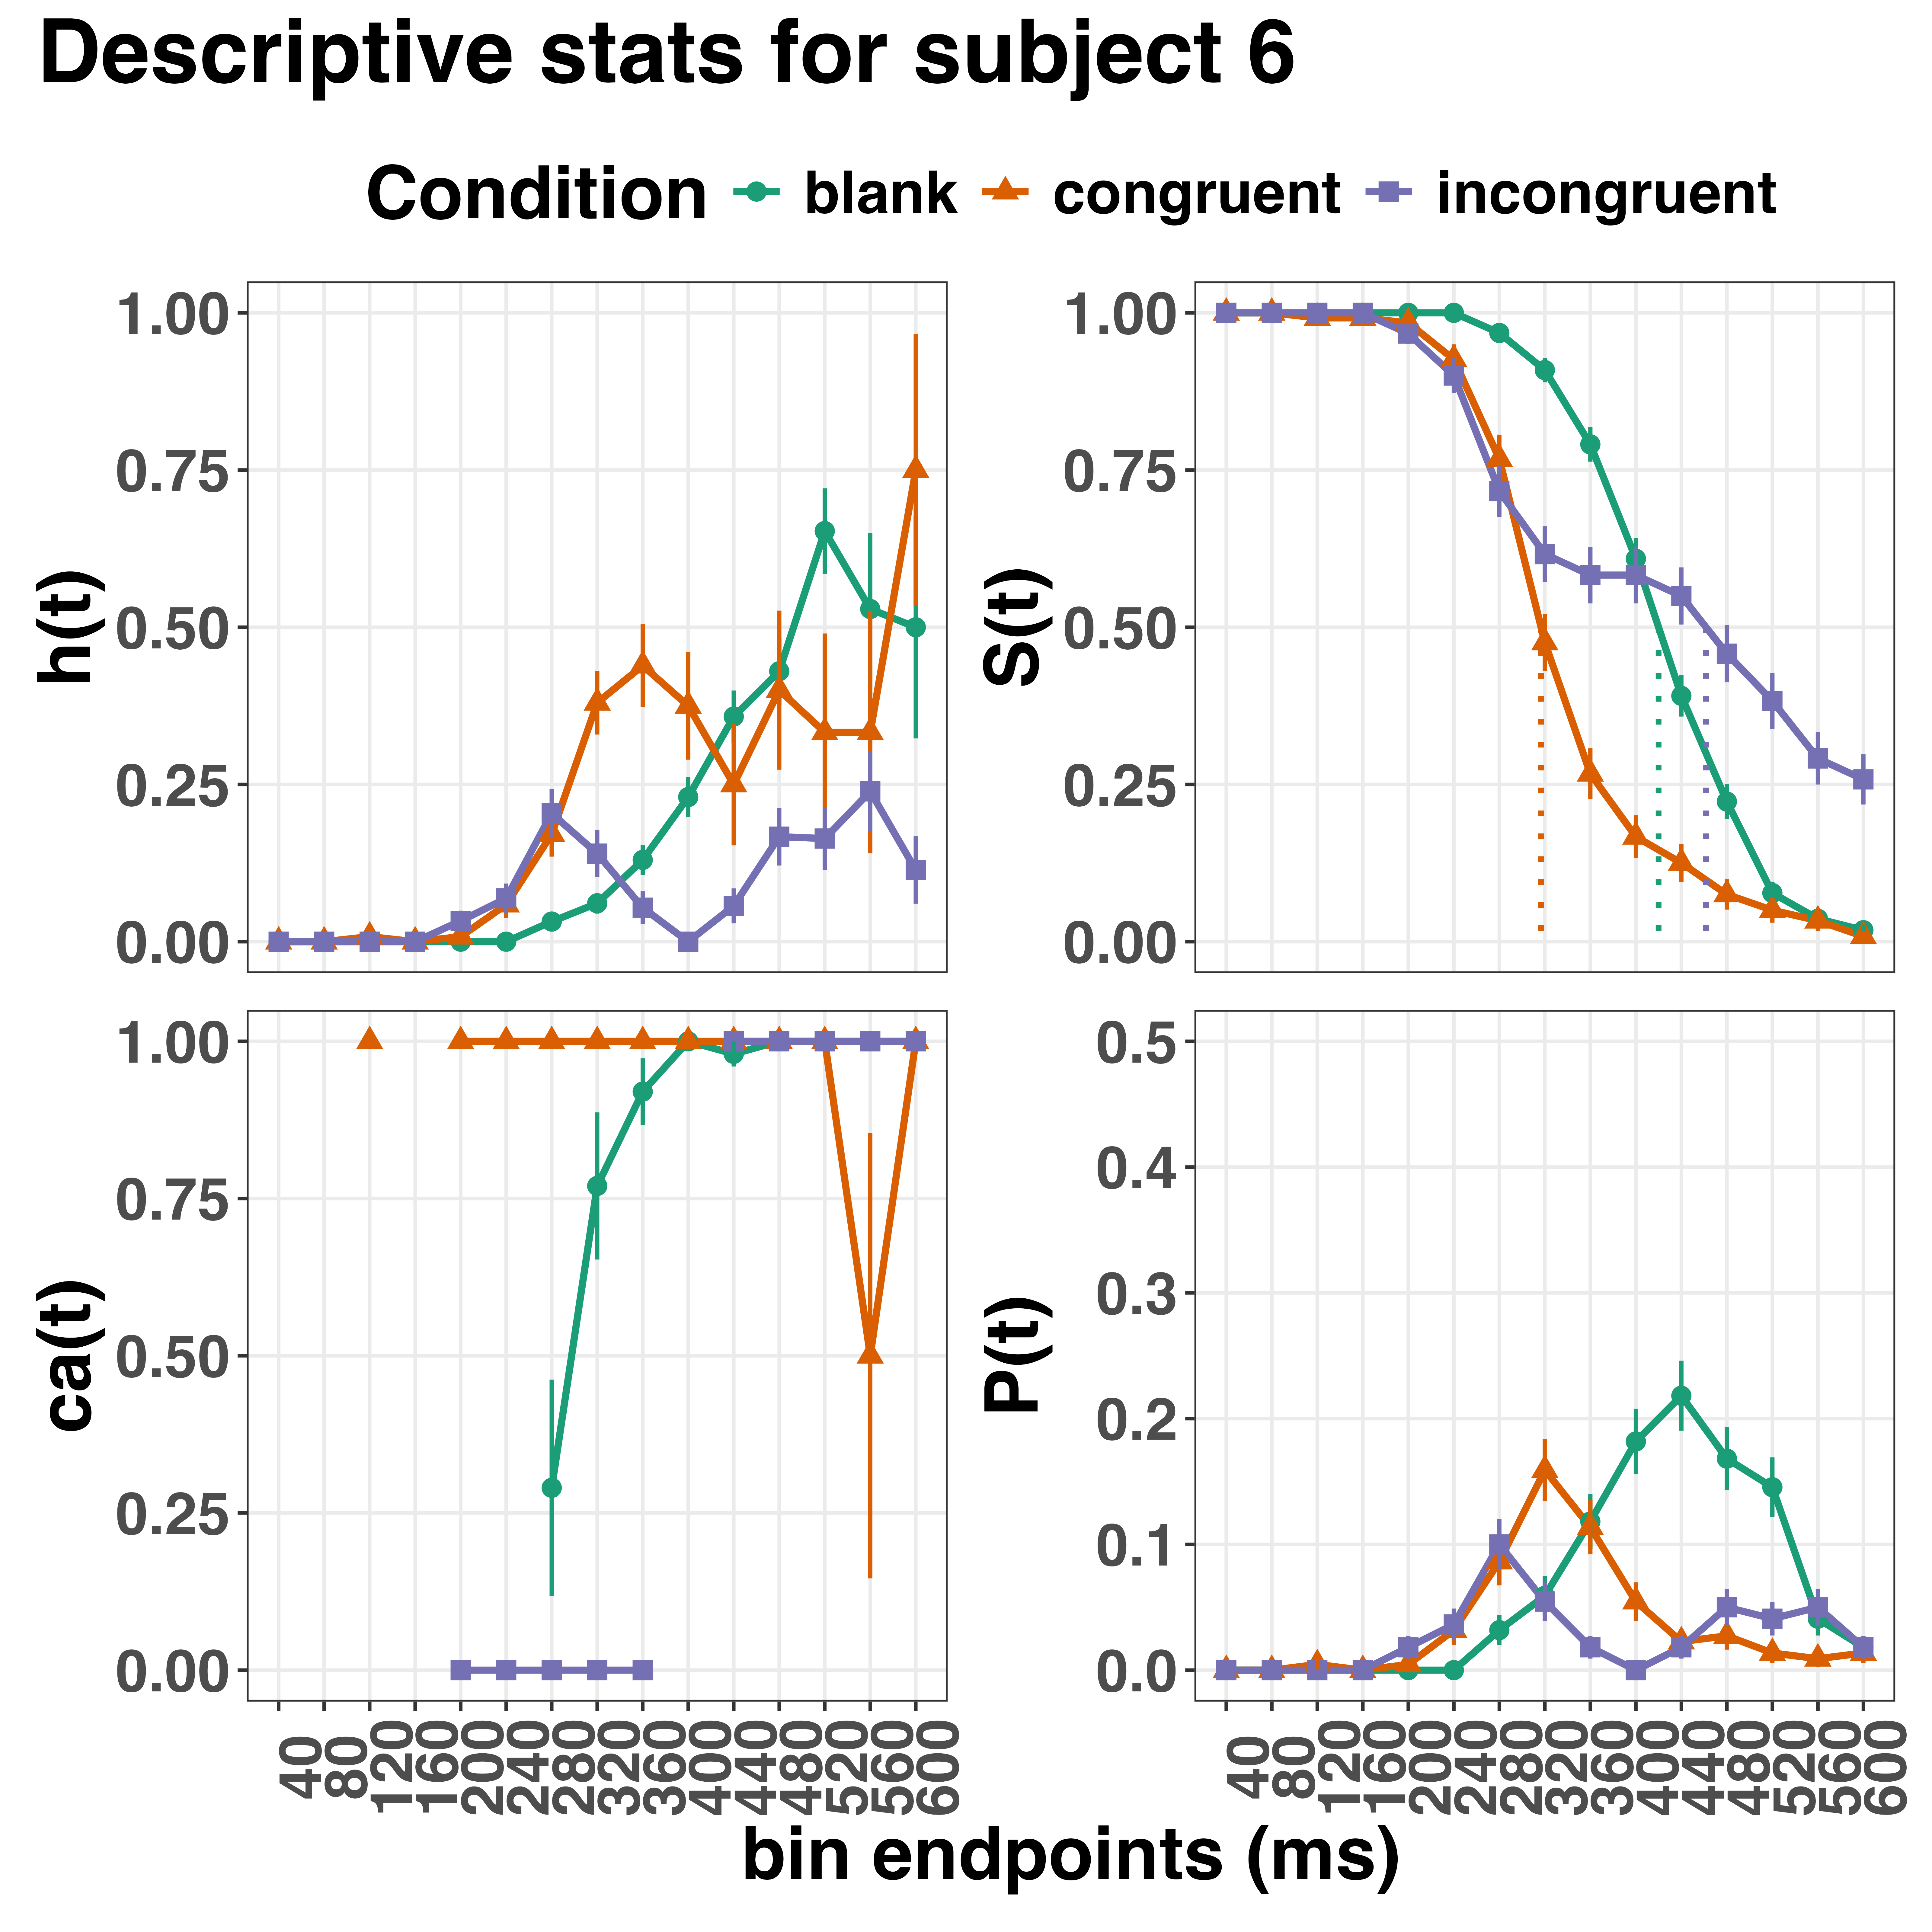
\includegraphics[width=12in,height=0.67\textheight,]{../Tutorial_1_descriptive_stats/figures/Plot_for_subject6_PanisSchmidt} 

}

\caption{Estimated discrete-time hazard, survivor, and conditional accuracy functions for participant 6, as a function of the passage of discrete waiting time.}\label{fig:eha-plot}
\end{figure}

However, when the waiting time has increased until \emph{400 ms} after target onset, then the conditional probability of response occurrence in the next 40 ms is estimated to be 0.36, 0.25, and 0.06 for the blank, congruent, and incongruent prime conditions, respectively. And when a response does occur in bin (400,440{]}, then the probability that it is correct is estimated to be 0.98, 1, and 1 for the blank, congruent, and incongruent prime conditions, respectively.

When participants show qualitatively the same distributional patterns, on might consider to aggregate their data and make one plot (see Tutorial\_1a.Rmd).

These results suggest that the participant is initially responding to the prime even though (s)he was instructed to only respond to the target, that response competition emerges in the incongruent prime condition around 300 ms, and that only later response are fully controlled by the target stimulus. Qualitatively similar results were obtained for the other five participants. These results go against the (often implicit) assumption that all observed responses are primed responses to the target stimulus.

At this point, we have calculated, summarised and plotted descriptive statistics for the key variables in EHA. As we will show in Tutorials 2 and 3, statistical models for h(t) and ca(t) can be implemented as generalized linear mixed regression models predicting event occurrence (1/0) and accuracy (1/0) in each bin of a selected timewindow for analysis. As such, multi-level regression is what we turn to in those tutorials. But first we consider the descriptive stats for two independent variables.

\subsection{4.2 Tutorial 1b: Generalising to a more complex design}\label{tutorial-1b-generalising-to-a-more-complex-design}

So far in this paper, we have use a simple experimental design, which involved one condition with two levels. But psychological experiments are often more complex, with crossed factorial designs with more conditions and more than two levels. The purpose of Tutorial 1b, therefore, is to provide a generalisation of the basic approach, which extends to a more complicated design. We felt that this might be useful for researchers in experimental psychology that typically use crossed factorial designs.

To this end, Tutorial 1b illustrates how to calculate and plot the descriptive statistics for the full data set of Experiment 1 of Panis and Schmidt (2016), which includes two independent variables: mask type and prime type. As we use the same functional programming approach as in Tutorial 1a, we simply present the sample-based functions for participant 6 in Figure 8.

Compared to the no-mask condition (column 1 in Figure 8), there is a negative compatibility effect in the hazard and conditional accuracy functions when a (relevant, irrelevant, or lines) mask is present.
T\ldots{}



\begin{figure}[H]

{\centering \includegraphics[width=0.95\linewidth,height=0.67\textheight,]{../Tutorial_1_descriptive_stats/figures/Plot_2IV_for_subject6_PanisSchmidt} 

}

\caption{Sample-based discrete-time hazard, survivor, and conditional accuracy functions for participant 6, as a function of prime type (blank, congruent, incongruent) and mask type (no mask, relevant, irrelevant, lines).}\label{fig:plot-2ivs}
\end{figure}

\subsection{4.3 Tutorial 2a: Fitting Bayesian hazard models}\label{tutorial-2a-fitting-bayesian-hazard-models}

In this third tutorial, we illustrate how to fit Bayesian hazard regression models to the masked response priming data set used in the first tutorial. Fitting (Bayesian or non-Bayesian) regression models to the data is important when you want to study how the shape of the hazard function depends on various predictors (Singer \& Willett, 2003).

\subsubsection{4.3.1 Hazard model considerations}\label{hazard-model-considerations}

There are several analytic decisions one has to make when fitting a hazard model. First, one has to select an analysis time window, i.e., a contiguous set of bins for which there is enough data for each participant. Second, given that the dependent variable is binary, one has to select a link function (see Supps). The cloglog link is preferred over the logit link when events can occur in principle at any time point within a bin, which is the case for RT data (Singer \& Willett, 2003). Third, one has to choose a specification of the effect of discrete TIME (i.e., the time bin index t). One can choose a general specification (one intercept per bin) or a functional specification, such as a polynomial one (compare model 1 with models 2, 3, and 4 below). We provide relevant example regression formulas in supplementary materials.

In the case of a large-\emph{N} design without repeated measurements, the parameters of a discrete-time hazard model can be estimated using standard logistic regression software after expanding the typical person-trial-oriented data set into a person-trial-bin-oriented data set (Allison, 2010). When there is clustering in the data, as in the case of a small-\emph{N} design with repeated measurements, the parameters of a discrete-time hazard model can be estimated using population-averaged methods (e.g., Generalized Estimating Equations), and Bayesian or frequentist generalized linear mixed models (Allison, 2010).

In general, there are three assumptions one can make or relax when adding experimental predictor variables and other covariates: The linearity assumption for continuous predictors (the effect of a 1 unit change is the same anywhere on the scale), the additivity assumption (predictors do not interact), and the proportionality assumption (predictors do not interact with TIME).

In this tutorial we will fit four Bayesian multilevel models (i.e., generalized linear mixed models) to the person-trial-bin oriented data set that we created in Tutorial 1a. We select the analysis range (200,600{]} and the cloglog link. The data is prepared as follows.

\scriptsize

\begin{Shaded}
\begin{Highlighting}[]
\CommentTok{\# load person{-}trial{-}bin oriented data set}
\NormalTok{ptb\_data }\OtherTok{\textless{}{-}} \FunctionTok{read\_csv}\NormalTok{(}\StringTok{"../Tutorial\_1\_descriptive\_stats/data/inputfile\_hazard\_modeling.csv"}\NormalTok{)}

\CommentTok{\# select analysis time range: (200,600] with 10 bins (time bin ranks 6 to 15)}
\NormalTok{ptb\_data }\OtherTok{\textless{}{-}}\NormalTok{ ptb\_data }\SpecialCharTok{\%\textgreater{}\%} \FunctionTok{filter}\NormalTok{(period }\SpecialCharTok{\textgreater{}} \DecValTok{5}\NormalTok{)}

\CommentTok{\# create factor condition, with "blank" as the reference level}
\NormalTok{ptb\_data }\OtherTok{\textless{}{-}}\NormalTok{ ptb\_data }\SpecialCharTok{\%\textgreater{}\%} \FunctionTok{mutate}\NormalTok{(}\AttributeTok{condition =} \FunctionTok{factor}\NormalTok{(condition, }\AttributeTok{labels =} \FunctionTok{c}\NormalTok{(}\StringTok{"blank"}\NormalTok{, }\StringTok{"congruent"}\NormalTok{,}\StringTok{"incongruent"}\NormalTok{)))}

\CommentTok{\# center TIME (period) on bin 9, and trial on trial 1000 and rescale; Add dummy variables for each bin.}
\NormalTok{ptb\_data }\OtherTok{\textless{}{-}}\NormalTok{ ptb\_data }\SpecialCharTok{\%\textgreater{}\%} 
        \FunctionTok{mutate}\NormalTok{(}\AttributeTok{period\_9 =}\NormalTok{ period }\SpecialCharTok{{-}} \DecValTok{9}\NormalTok{,}
               \AttributeTok{trial\_c =}\NormalTok{ (trial }\SpecialCharTok{{-}} \DecValTok{1000}\NormalTok{)}\SpecialCharTok{/}\DecValTok{1000}\NormalTok{,}
               \AttributeTok{d6  =} \FunctionTok{if\_else}\NormalTok{(period }\SpecialCharTok{==} \DecValTok{6}\NormalTok{, }\DecValTok{1}\NormalTok{, }\DecValTok{0}\NormalTok{),}
               \AttributeTok{d7  =} \FunctionTok{if\_else}\NormalTok{(period }\SpecialCharTok{==} \DecValTok{7}\NormalTok{, }\DecValTok{1}\NormalTok{, }\DecValTok{0}\NormalTok{),}
               \AttributeTok{d8  =} \FunctionTok{if\_else}\NormalTok{(period }\SpecialCharTok{==} \DecValTok{8}\NormalTok{, }\DecValTok{1}\NormalTok{, }\DecValTok{0}\NormalTok{),}
               \AttributeTok{d9  =} \FunctionTok{if\_else}\NormalTok{(period }\SpecialCharTok{==} \DecValTok{9}\NormalTok{, }\DecValTok{1}\NormalTok{, }\DecValTok{0}\NormalTok{),}
               \AttributeTok{d10 =} \FunctionTok{if\_else}\NormalTok{(period }\SpecialCharTok{==} \DecValTok{10}\NormalTok{, }\DecValTok{1}\NormalTok{, }\DecValTok{0}\NormalTok{),}
               \AttributeTok{d11 =} \FunctionTok{if\_else}\NormalTok{(period }\SpecialCharTok{==} \DecValTok{11}\NormalTok{, }\DecValTok{1}\NormalTok{, }\DecValTok{0}\NormalTok{),}
               \AttributeTok{d12 =} \FunctionTok{if\_else}\NormalTok{(period }\SpecialCharTok{==} \DecValTok{12}\NormalTok{, }\DecValTok{1}\NormalTok{, }\DecValTok{0}\NormalTok{),}
               \AttributeTok{d13 =} \FunctionTok{if\_else}\NormalTok{(period }\SpecialCharTok{==} \DecValTok{13}\NormalTok{, }\DecValTok{1}\NormalTok{, }\DecValTok{0}\NormalTok{),}
               \AttributeTok{d14 =} \FunctionTok{if\_else}\NormalTok{(period }\SpecialCharTok{==} \DecValTok{14}\NormalTok{, }\DecValTok{1}\NormalTok{, }\DecValTok{0}\NormalTok{),}
               \AttributeTok{d15 =} \FunctionTok{if\_else}\NormalTok{(period }\SpecialCharTok{==} \DecValTok{15}\NormalTok{, }\DecValTok{1}\NormalTok{, }\DecValTok{0}\NormalTok{))}
\end{Highlighting}
\end{Shaded}

\normalsize

\subsubsection{4.3.2 Prior distributions}\label{prior-distributions}

To get the posterior distribution of each parameters given the data, we need to specify a prior distribution for each parameter. The middle column of Supplementary Figure 4 shows seven examples of prior distributions on the logit and/or cloglog scales.

While a normal distribution with relatively large variance is often used as a weakly informative prior for continuous dependent variables, rows A and B in Figure 3 show that specifying such distributions on the logit and cloglog scales leads to rather informative distributions on the original probability (i.e., discrete-time hazard) scale, as most mass is pushed to probabilities of 0 and 1.

\subsubsection{4.3.3 Model 1: A general specification of TIME, and main effects of congruency and trial number}\label{model-1-a-general-specification-of-time-and-main-effects-of-congruency-and-trial-number}

{[}{[}Here let's give some intuition on why we would want to setup the model like this{]}{]}

For the first model, we use a general specification of TIME (i.e., one intercept per time bin) for the baseline condition (blank prime), and assume that the effects of prime-target congruency and trial number are proportional and additive, and that the effect of trial number is linear.
Before we fit model 1, we remove unnecessary columns from the data, and specify our priors. In the code of Tutorial 2, this is accomplished as follows.

\scriptsize

\begin{Shaded}
\begin{Highlighting}[]
\CommentTok{\# remove unnecessary columns before fitting a model}
\NormalTok{M1\_data }\OtherTok{\textless{}{-}}\NormalTok{ ptb\_data }\SpecialCharTok{\%\textgreater{}\%} \FunctionTok{select}\NormalTok{(}\SpecialCharTok{{-}}\FunctionTok{c}\NormalTok{(bl,tr,trial,period, period\_9,d9))  }

\CommentTok{\# Specify priors}
\NormalTok{priors\_M1 }\OtherTok{\textless{}{-}} \FunctionTok{c}\NormalTok{(}
  \FunctionTok{set\_prior}\NormalTok{(}\StringTok{"skew\_normal({-}0.2,0.71,{-}2.2)"}\NormalTok{, }\AttributeTok{class =} \StringTok{"b"}\NormalTok{),       }
  \FunctionTok{set\_prior}\NormalTok{(}\StringTok{"skew\_normal({-}1,1,{-}2)"}\NormalTok{, }\AttributeTok{class =} \StringTok{"b"}\NormalTok{, }\AttributeTok{coef =} \StringTok{"d6"}\NormalTok{),}
  \FunctionTok{set\_prior}\NormalTok{(}\StringTok{"skew\_normal({-}1,1,{-}2)"}\NormalTok{, }\AttributeTok{class =} \StringTok{"b"}\NormalTok{, }\AttributeTok{coef =} \StringTok{"d7"}\NormalTok{), }
  \FunctionTok{set\_prior}\NormalTok{(}\StringTok{"skew\_normal({-}1,1,{-}2)"}\NormalTok{, }\AttributeTok{class =} \StringTok{"b"}\NormalTok{, }\AttributeTok{coef =} \StringTok{"d8"}\NormalTok{), }
  \FunctionTok{set\_prior}\NormalTok{(}\StringTok{"skew\_normal({-}1,1,{-}2)"}\NormalTok{, }\AttributeTok{class =} \StringTok{"b"}\NormalTok{, }\AttributeTok{coef =} \StringTok{"d10"}\NormalTok{), }
  \FunctionTok{set\_prior}\NormalTok{(}\StringTok{"skew\_normal({-}1,1,{-}2)"}\NormalTok{, }\AttributeTok{class =} \StringTok{"b"}\NormalTok{, }\AttributeTok{coef =} \StringTok{"d11"}\NormalTok{), }
  \FunctionTok{set\_prior}\NormalTok{(}\StringTok{"skew\_normal({-}1,1,{-}2)"}\NormalTok{, }\AttributeTok{class =} \StringTok{"b"}\NormalTok{, }\AttributeTok{coef =} \StringTok{"d12"}\NormalTok{), }
  \FunctionTok{set\_prior}\NormalTok{(}\StringTok{"skew\_normal({-}1,1,{-}2)"}\NormalTok{, }\AttributeTok{class =} \StringTok{"b"}\NormalTok{, }\AttributeTok{coef =} \StringTok{"d13"}\NormalTok{), }
  \FunctionTok{set\_prior}\NormalTok{(}\StringTok{"skew\_normal({-}1,1,{-}2)"}\NormalTok{, }\AttributeTok{class =} \StringTok{"b"}\NormalTok{, }\AttributeTok{coef =} \StringTok{"d14"}\NormalTok{), }
  \FunctionTok{set\_prior}\NormalTok{(}\StringTok{"skew\_normal({-}1,1,{-}2)"}\NormalTok{, }\AttributeTok{class =} \StringTok{"b"}\NormalTok{, }\AttributeTok{coef =} \StringTok{"d15"}\NormalTok{),}
  \FunctionTok{set\_prior}\NormalTok{(}\StringTok{"skew\_normal({-}1,1,{-}2)"}\NormalTok{, }\AttributeTok{class =} \StringTok{"b"}\NormalTok{, }\AttributeTok{coef =} \StringTok{"Intercept"}\NormalTok{),}
  \FunctionTok{set\_prior}\NormalTok{(}\StringTok{"normal(0, 1)"}\NormalTok{, }\AttributeTok{class =} \StringTok{"sd"}\NormalTok{),        }
  \FunctionTok{set\_prior}\NormalTok{(}\StringTok{"lkj(2)"}\NormalTok{, }\AttributeTok{class =} \StringTok{"cor"}\NormalTok{)            }
\NormalTok{)}
\end{Highlighting}
\end{Shaded}

\normalsize

We can now estimate our first Bayesion regression model, as follows.

\scriptsize

\begin{Shaded}
\begin{Highlighting}[]
\FunctionTok{plan}\NormalTok{(multicore)}

\NormalTok{model\_M1 }\OtherTok{\textless{}{-}}
   \FunctionTok{brm}\NormalTok{(}\AttributeTok{data =}\NormalTok{ M1\_data,}
       \AttributeTok{family =} \FunctionTok{binomial}\NormalTok{(}\AttributeTok{link=}\StringTok{"cloglog"}\NormalTok{),}
\NormalTok{       event }\SpecialCharTok{|} \FunctionTok{trials}\NormalTok{(}\DecValTok{1}\NormalTok{) }\SpecialCharTok{\textasciitilde{}} \DecValTok{0} \SpecialCharTok{+}\NormalTok{ d6 }\SpecialCharTok{+}\NormalTok{ d7 }\SpecialCharTok{+}\NormalTok{ d8 }\SpecialCharTok{+}\NormalTok{ Intercept }\SpecialCharTok{+}\NormalTok{ d10 }\SpecialCharTok{+}\NormalTok{ d11 }\SpecialCharTok{+}\NormalTok{ d12 }\SpecialCharTok{+}\NormalTok{ d13 }\SpecialCharTok{+}\NormalTok{ d14 }\SpecialCharTok{+}\NormalTok{ d15 }\SpecialCharTok{+} 
\NormalTok{         condition }\SpecialCharTok{+}\NormalTok{ trial\_c }\SpecialCharTok{+}
       
\NormalTok{                   (d6 }\SpecialCharTok{+}\NormalTok{ d7 }\SpecialCharTok{+}\NormalTok{ d8 }\SpecialCharTok{+} \DecValTok{1} \SpecialCharTok{+}\NormalTok{ d10 }\SpecialCharTok{+}\NormalTok{ d11 }\SpecialCharTok{+}\NormalTok{ d12 }\SpecialCharTok{+}\NormalTok{ d13 }\SpecialCharTok{+}\NormalTok{ d14 }\SpecialCharTok{+}\NormalTok{ d15 }\SpecialCharTok{+}\NormalTok{ condition }\SpecialCharTok{+}\NormalTok{ trial\_c }\SpecialCharTok{|}\NormalTok{ pid),}
       \AttributeTok{prior =}\NormalTok{ priors\_M1,}
       \AttributeTok{chains =} \DecValTok{4}\NormalTok{, }\AttributeTok{cores =} \DecValTok{4}\NormalTok{, }\AttributeTok{iter =} \DecValTok{3000}\NormalTok{, }\AttributeTok{warmup =} \DecValTok{1000}\NormalTok{,}
       \AttributeTok{control =} \FunctionTok{list}\NormalTok{(}\AttributeTok{adapt\_delta =} \FloatTok{0.999}\NormalTok{, }\AttributeTok{step\_size =} \FloatTok{0.04}\NormalTok{, }\AttributeTok{max\_treedepth =} \DecValTok{12}\NormalTok{),}
       \AttributeTok{seed =} \DecValTok{12}\NormalTok{, }\AttributeTok{init =} \StringTok{"0"}\NormalTok{,}
       \AttributeTok{file =} \StringTok{"Tutorial\_2\_Bayesian/models/model\_M1"}\NormalTok{)}
\end{Highlighting}
\end{Shaded}

\normalsize

Estimating model M1 took about 70 minutes on a MacBook Pro (Sonoma 14.6.1 OS, 18GB Memory, M3 Pro Chip).

\subsubsection{4.3.4 Model 2: A polynomial specification of TIME, and main effects of congruency and trial number}\label{model-2-a-polynomial-specification-of-time-and-main-effects-of-congruency-and-trial-number}

{[}{[}Here let's give some intuition on why we would want to modify the formula and model features{]}{]}

For the second model, we use a third-order polynomial specification of TIME for the baseline condition (blank prime), and again assume that the effects of prime-target congruency and trial number are proportional and additive, and that the effect of trial number is linear. We first remove unncessary columns and specify our priors.

Estimating model M2 took about 144 minutes.

\subsubsection{4.3.5 Model 3: A polynomial specification of TIME, and relaxing the proportionality assumption}\label{model-3-a-polynomial-specification-of-time-and-relaxing-the-proportionality-assumption}

{[}{[}Here let's give some intuition on why we would want to modify the formula and model features{]}{]}

For the third model, we use a third-order polynomial specification of TIME for the baseline condition (blank prime), and relax the proportionality assumption for the predictor variables congruency (variable ``condition'') and trial number (variable ``trial\_c''). We use the same data set and priors as for model 2.

Estimating model M3 took about 268 minutes.

\subsubsection{4.3.6 Model 4: A polynomial specification of TIME, and relaxing all three assumptions}\label{model-4-a-polynomial-specification-of-time-and-relaxing-all-three-assumptions}

Based on previous work (Panis, 2020; Panis, Moran, Wolkersdorfer, \& Schmidt, 2020; Panis \& Schmidt, 2022; Panis, Torfs, Gillebert, Wagemans, \& Humphreys, 2017; Panis \& Wagemans, 2009), we relax all three assumptions in model 4. We use the same data set and priors as for model 2.

Estimating model M4 took about 8 hours.

\subsubsection{4.3.7 Compare the models.}\label{compare-the-models.}

We can compare the four models using the Widely Applicable Information Criterion (WAIC) and Leave-One-Out (LOO) cross-validation, and look at model weights (Kurz, 2023a; McElreath, 2018).

Clearly, both weighting schemes prefer model M4.

\subsubsection{4.3.8 Evaluate parameter estimates}\label{evaluate-parameter-estimates}

Figure 5 shows the effects of congruent and incongruent primes relative to neutral primes, for each time bin in trial numbers 500, 1000, and 1500 for the selected model.



\begin{figure}[H]

{\centering 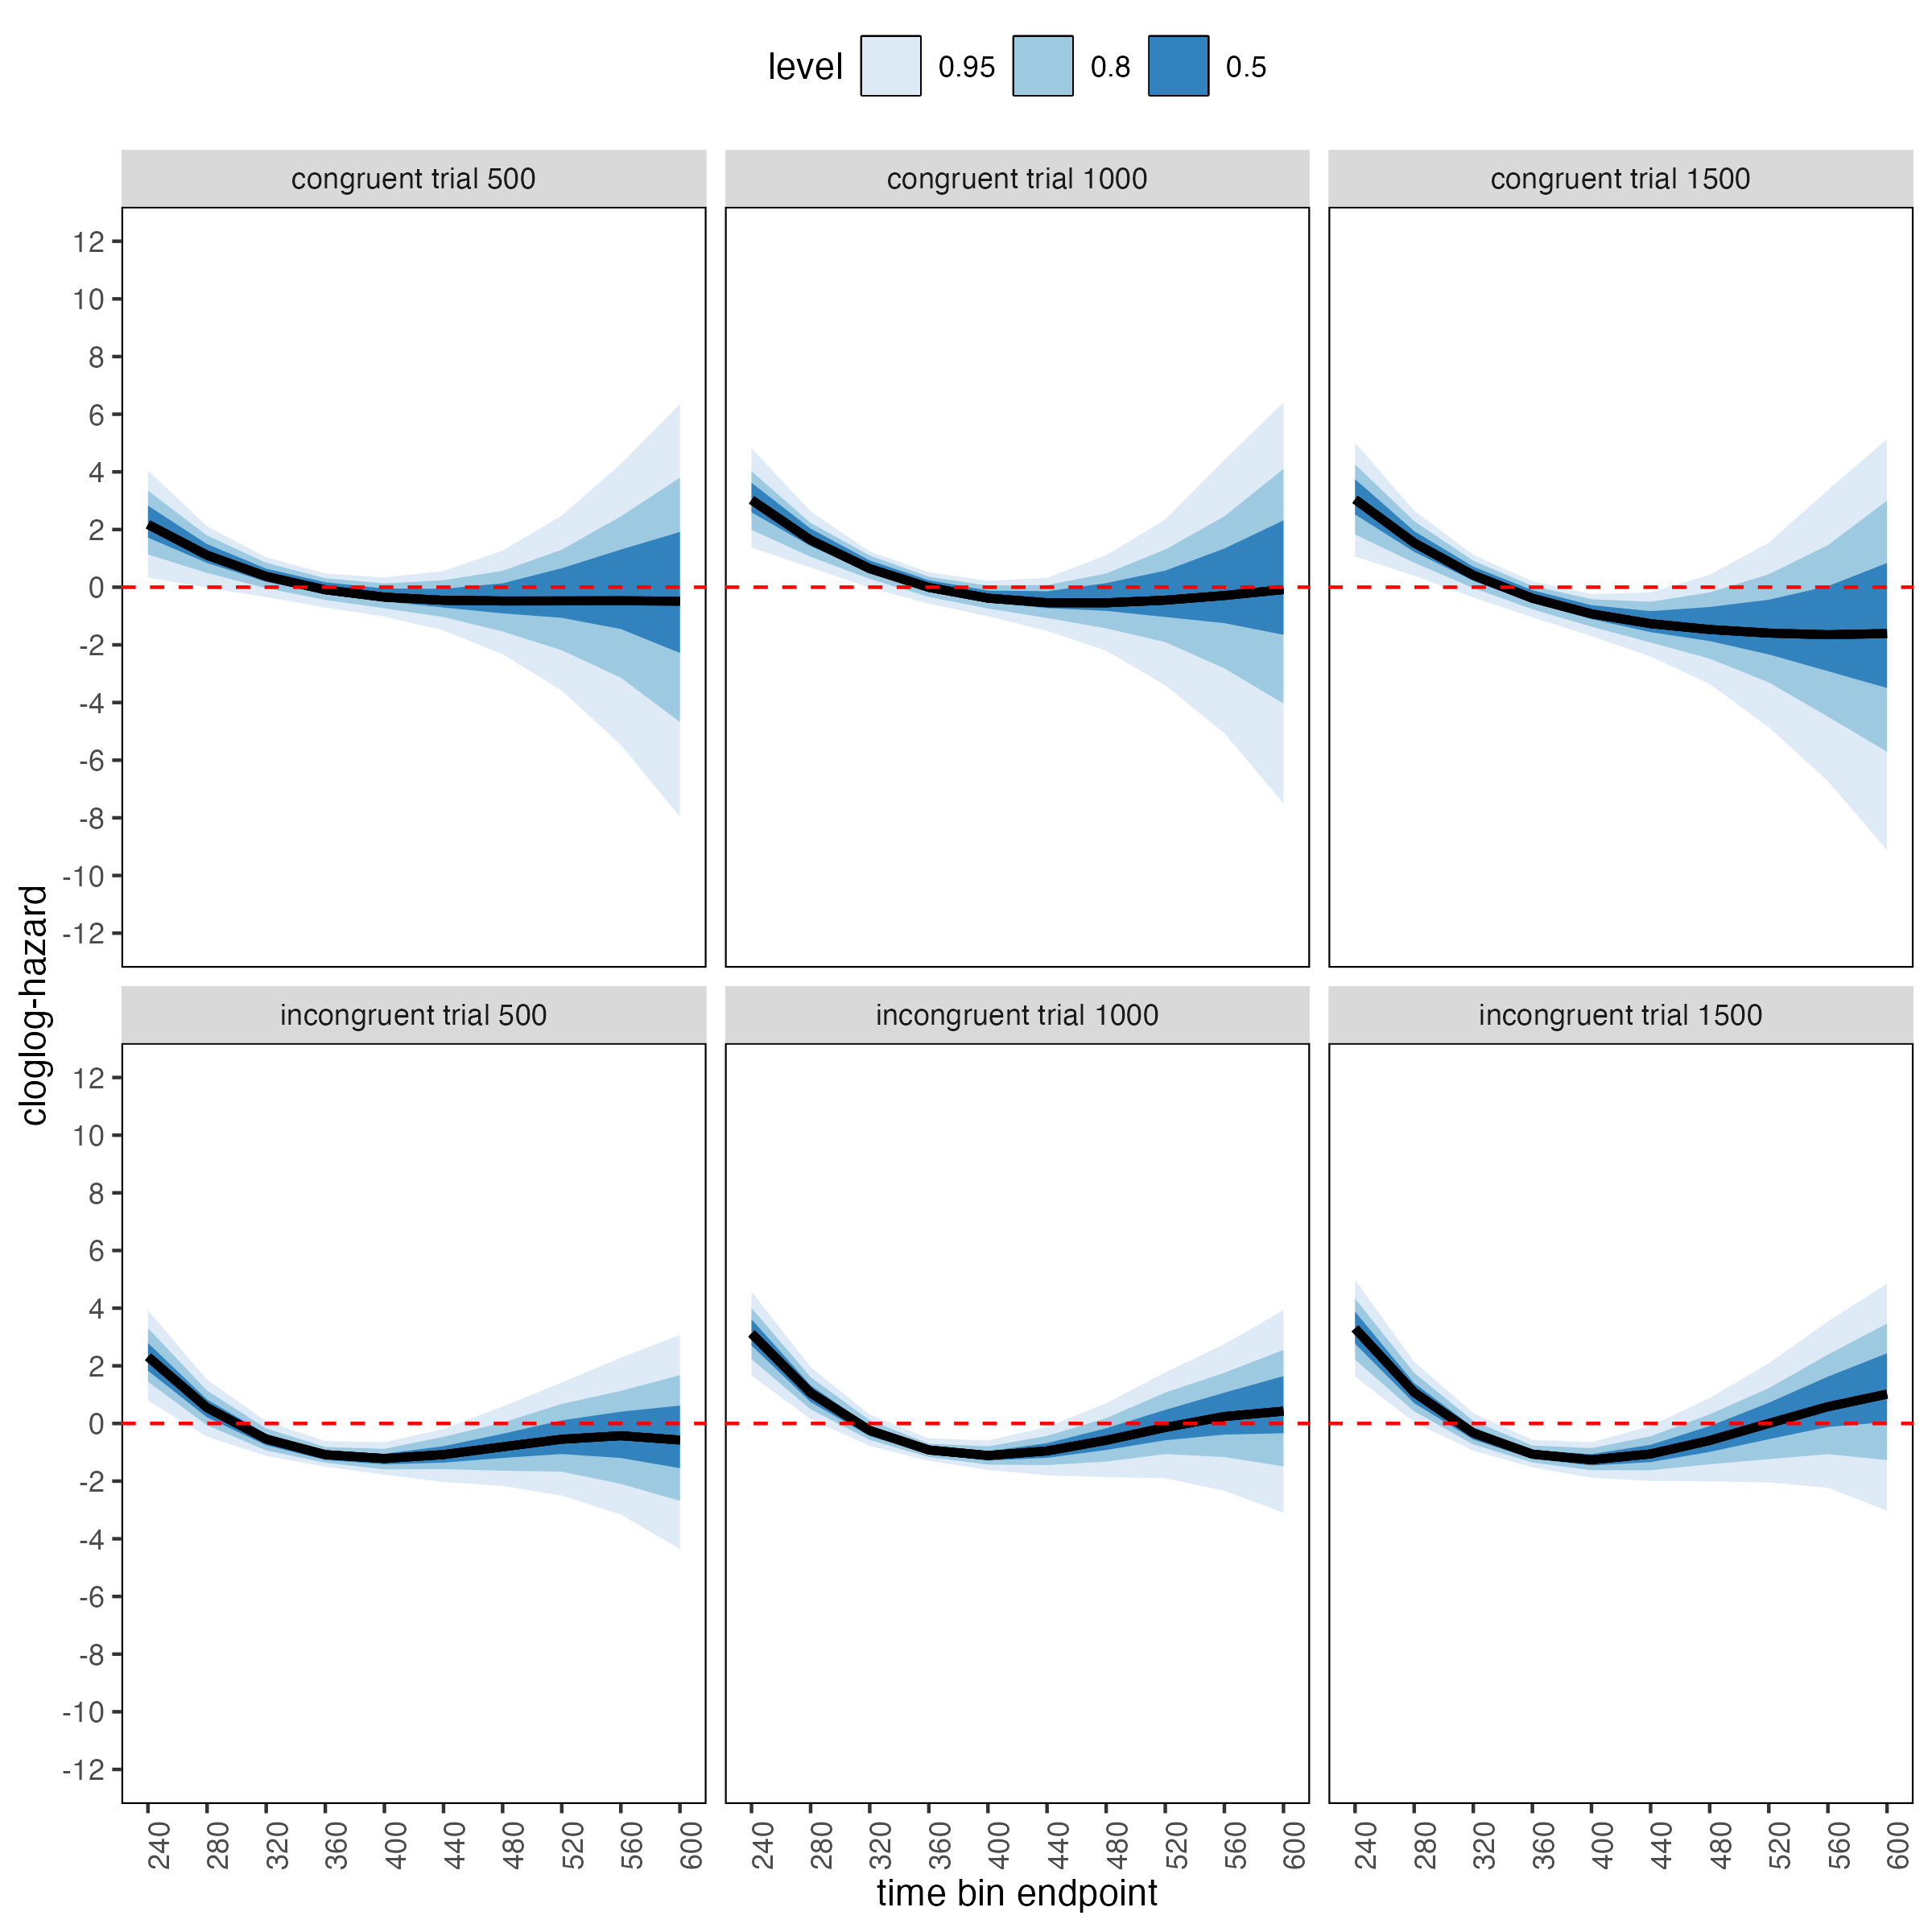
\includegraphics[width=0.8\linewidth,height=0.67\textheight,]{../Tutorial_2_Bayesian/figures/M4effects_con_incon_3trials} 

}

\caption{50/80/95 percentile intervals of the draws from the posterior distributions representing the effect of congruent and incongruent primes relative to neutral primes in trial number 1000.}\label{fig:plot-prime-effects}
\end{figure}

Tabel X shows the mean point estimates and the upper and lower limits of the 95\% highest density intervals for each bin





\begin{center}
\begin{ThreePartTable}

\begin{TableNotes}[para]
\normalsize{\textit{Note.} The posterior distributions of the effects of congruent and incongruent primes relative to no primes are summarized by point estimates and the lower and upper \ldots{}}
\end{TableNotes}

\scriptsize{

\begin{longtable}{lllllll}\noalign{\getlongtablewidth\global\LTcapwidth=\longtablewidth}
\caption{\label{tab:int-table}Point and interval estimates.}\\
\toprule
bin\_endpoint & \multicolumn{1}{c}{condition} & \multicolumn{1}{c}{mean} & \multicolumn{1}{c}{.lower} & \multicolumn{1}{c}{.upper} & \multicolumn{1}{c}{.width} & \multicolumn{1}{c}{hazard ratio}\\
\midrule
\endfirsthead
\caption*{\normalfont{Table \ref{tab:int-table} continued}}\\
\toprule
bin\_endpoint & \multicolumn{1}{c}{condition} & \multicolumn{1}{c}{mean} & \multicolumn{1}{c}{.lower} & \multicolumn{1}{c}{.upper} & \multicolumn{1}{c}{.width} & \multicolumn{1}{c}{hazard ratio}\\
\midrule
\endhead
240.00 & c500 & 2.18 & 0.33 & 4.05 & 0.95 & 8.82\\
280.00 & c500 & 1.11 & -0.02 & 2.11 & 0.95 & 3.03\\
320.00 & c500 & 0.37 & -0.34 & 1.04 & 0.95 & 1.45\\
360.00 & c500 & -0.09 & -0.70 & 0.48 & 0.95 & 0.91\\
400.00 & c500 & -0.35 & -1.02 & 0.34 & 0.95 & 0.71\\
440.00 & c500 & -0.45 & -1.50 & 0.56 & 0.95 & 0.64\\
480.00 & c500 & -0.48 & -2.32 & 1.27 & 0.95 & 0.62\\
520.00 & c500 & -0.48 & -3.57 & 2.52 & 0.95 & 0.62\\
560.00 & c500 & -0.52 & -5.69 & 4.27 & 0.95 & 0.60\\
600.00 & c500 & -0.66 & -8.56 & 6.99 & 0.95 & 0.52\\
240.00 & c1000 & 3.03 & 1.37 & 4.82 & 0.95 & 20.63\\
280.00 & c1000 & 1.63 & 0.68 & 2.63 & 0.95 & 5.13\\
320.00 & c1000 & 0.64 & -0.02 & 1.24 & 0.95 & 1.90\\
360.00 & c1000 & -0.01 & -0.57 & 0.52 & 0.95 & 0.99\\
400.00 & c1000 & -0.38 & -1.01 & 0.22 & 0.95 & 0.68\\
440.00 & c1000 & -0.54 & -1.52 & 0.32 & 0.95 & 0.58\\
480.00 & c1000 & -0.54 & -2.20 & 1.11 & 0.95 & 0.58\\
520.00 & c1000 & -0.45 & -3.40 & 2.35 & 0.95 & 0.64\\
560.00 & c1000 & -0.34 & -5.78 & 3.90 & 0.95 & 0.71\\
600.00 & c1000 & -0.25 & -8.34 & 6.73 & 0.95 & 0.78\\
240.00 & c1500 & 3.05 & 1.07 & 5.02 & 0.95 & 21.02\\
280.00 & c1500 & 1.54 & 0.40 & 2.65 & 0.95 & 4.66\\
320.00 & c1500 & 0.42 & -0.36 & 1.13 & 0.95 & 1.52\\
360.00 & c1500 & -0.38 & -1.05 & 0.21 & 0.95 & 0.68\\
400.00 & c1500 & -0.92 & -1.70 & -0.24 & 0.95 & 0.40\\
440.00 & c1500 & -1.26 & -2.41 & -0.18 & 0.95 & 0.28\\
480.00 & c1500 & -1.47 & -3.36 & 0.43 & 0.95 & 0.23\\
520.00 & c1500 & -1.60 & -4.86 & 1.58 & 0.95 & 0.20\\
560.00 & c1500 & -1.71 & -7.01 & 3.37 & 0.95 & 0.18\\
600.00 & c1500 & -1.88 & -10.07 & 5.98 & 0.95 & 0.15\\
240.00 & i500 & 2.31 & 0.79 & 3.93 & 0.95 & 10.10\\
280.00 & i500 & 0.55 & -0.46 & 1.52 & 0.95 & 1.72\\
320.00 & i500 & -0.54 & -1.13 & 0.08 & 0.95 & 0.58\\
360.00 & i500 & -1.08 & -1.50 & -0.61 & 0.95 & 0.34\\
400.00 & i500 & -1.22 & -1.78 & -0.65 & 0.95 & 0.30\\
440.00 & i500 & -1.08 & -2.03 & -0.19 & 0.95 & 0.34\\
480.00 & i500 & -0.81 & -2.16 & 0.59 & 0.95 & 0.44\\
520.00 & i500 & -0.55 & -2.50 & 1.42 & 0.95 & 0.58\\
560.00 & i500 & -0.42 & -3.16 & 2.28 & 0.95 & 0.65\\
600.00 & i500 & -0.58 & -4.35 & 3.10 & 0.95 & 0.56\\
240.00 & i1000 & 3.12 & 1.66 & 4.58 & 0.95 & 22.68\\
280.00 & i1000 & 1.06 & 0.15 & 1.95 & 0.95 & 2.88\\
320.00 & i1000 & -0.24 & -0.78 & 0.31 & 0.95 & 0.78\\
360.00 & i1000 & -0.92 & -1.30 & -0.52 & 0.95 & 0.40\\
400.00 & i1000 & -1.11 & -1.61 & -0.59 & 0.95 & 0.33\\
440.00 & i1000 & -0.95 & -1.80 & -0.12 & 0.95 & 0.39\\
480.00 & i1000 & -0.58 & -1.86 & 0.70 & 0.95 & 0.56\\
520.00 & i1000 & -0.14 & -1.90 & 1.77 & 0.95 & 0.87\\
560.00 & i1000 & 0.24 & -2.33 & 2.75 & 0.95 & 1.27\\
600.00 & i1000 & 0.42 & -3.17 & 3.85 & 0.95 & 1.52\\
240.00 & i1500 & 3.30 & 1.63 & 4.98 & 0.95 & 27.07\\
280.00 & i1500 & 1.08 & 0.05 & 2.14 & 0.95 & 2.94\\
320.00 & i1500 & -0.33 & -0.94 & 0.36 & 0.95 & 0.72\\
360.00 & i1500 & -1.06 & -1.52 & -0.57 & 0.95 & 0.35\\
400.00 & i1500 & -1.26 & -1.88 & -0.65 & 0.95 & 0.28\\
440.00 & i1500 & -1.06 & -1.99 & -0.09 & 0.95 & 0.35\\
480.00 & i1500 & -0.59 & -2.01 & 0.88 & 0.95 & 0.55\\
520.00 & i1500 & 0.00 & -2.05 & 2.09 & 0.95 & 1.00\\
560.00 & i1500 & 0.58 & -2.23 & 3.54 & 0.95 & 1.79\\
600.00 & i1500 & 1.01 & -3.02 & 4.86 & 0.95 & 2.75\\
\bottomrule
\addlinespace
\insertTableNotes
\end{longtable}

}

\end{ThreePartTable}
\end{center}

Figure 6 shows the model-based hazard functions for each prime type for participant 6, in trial 500, 1000, and 1500.



\begin{figure}[H]

{\centering 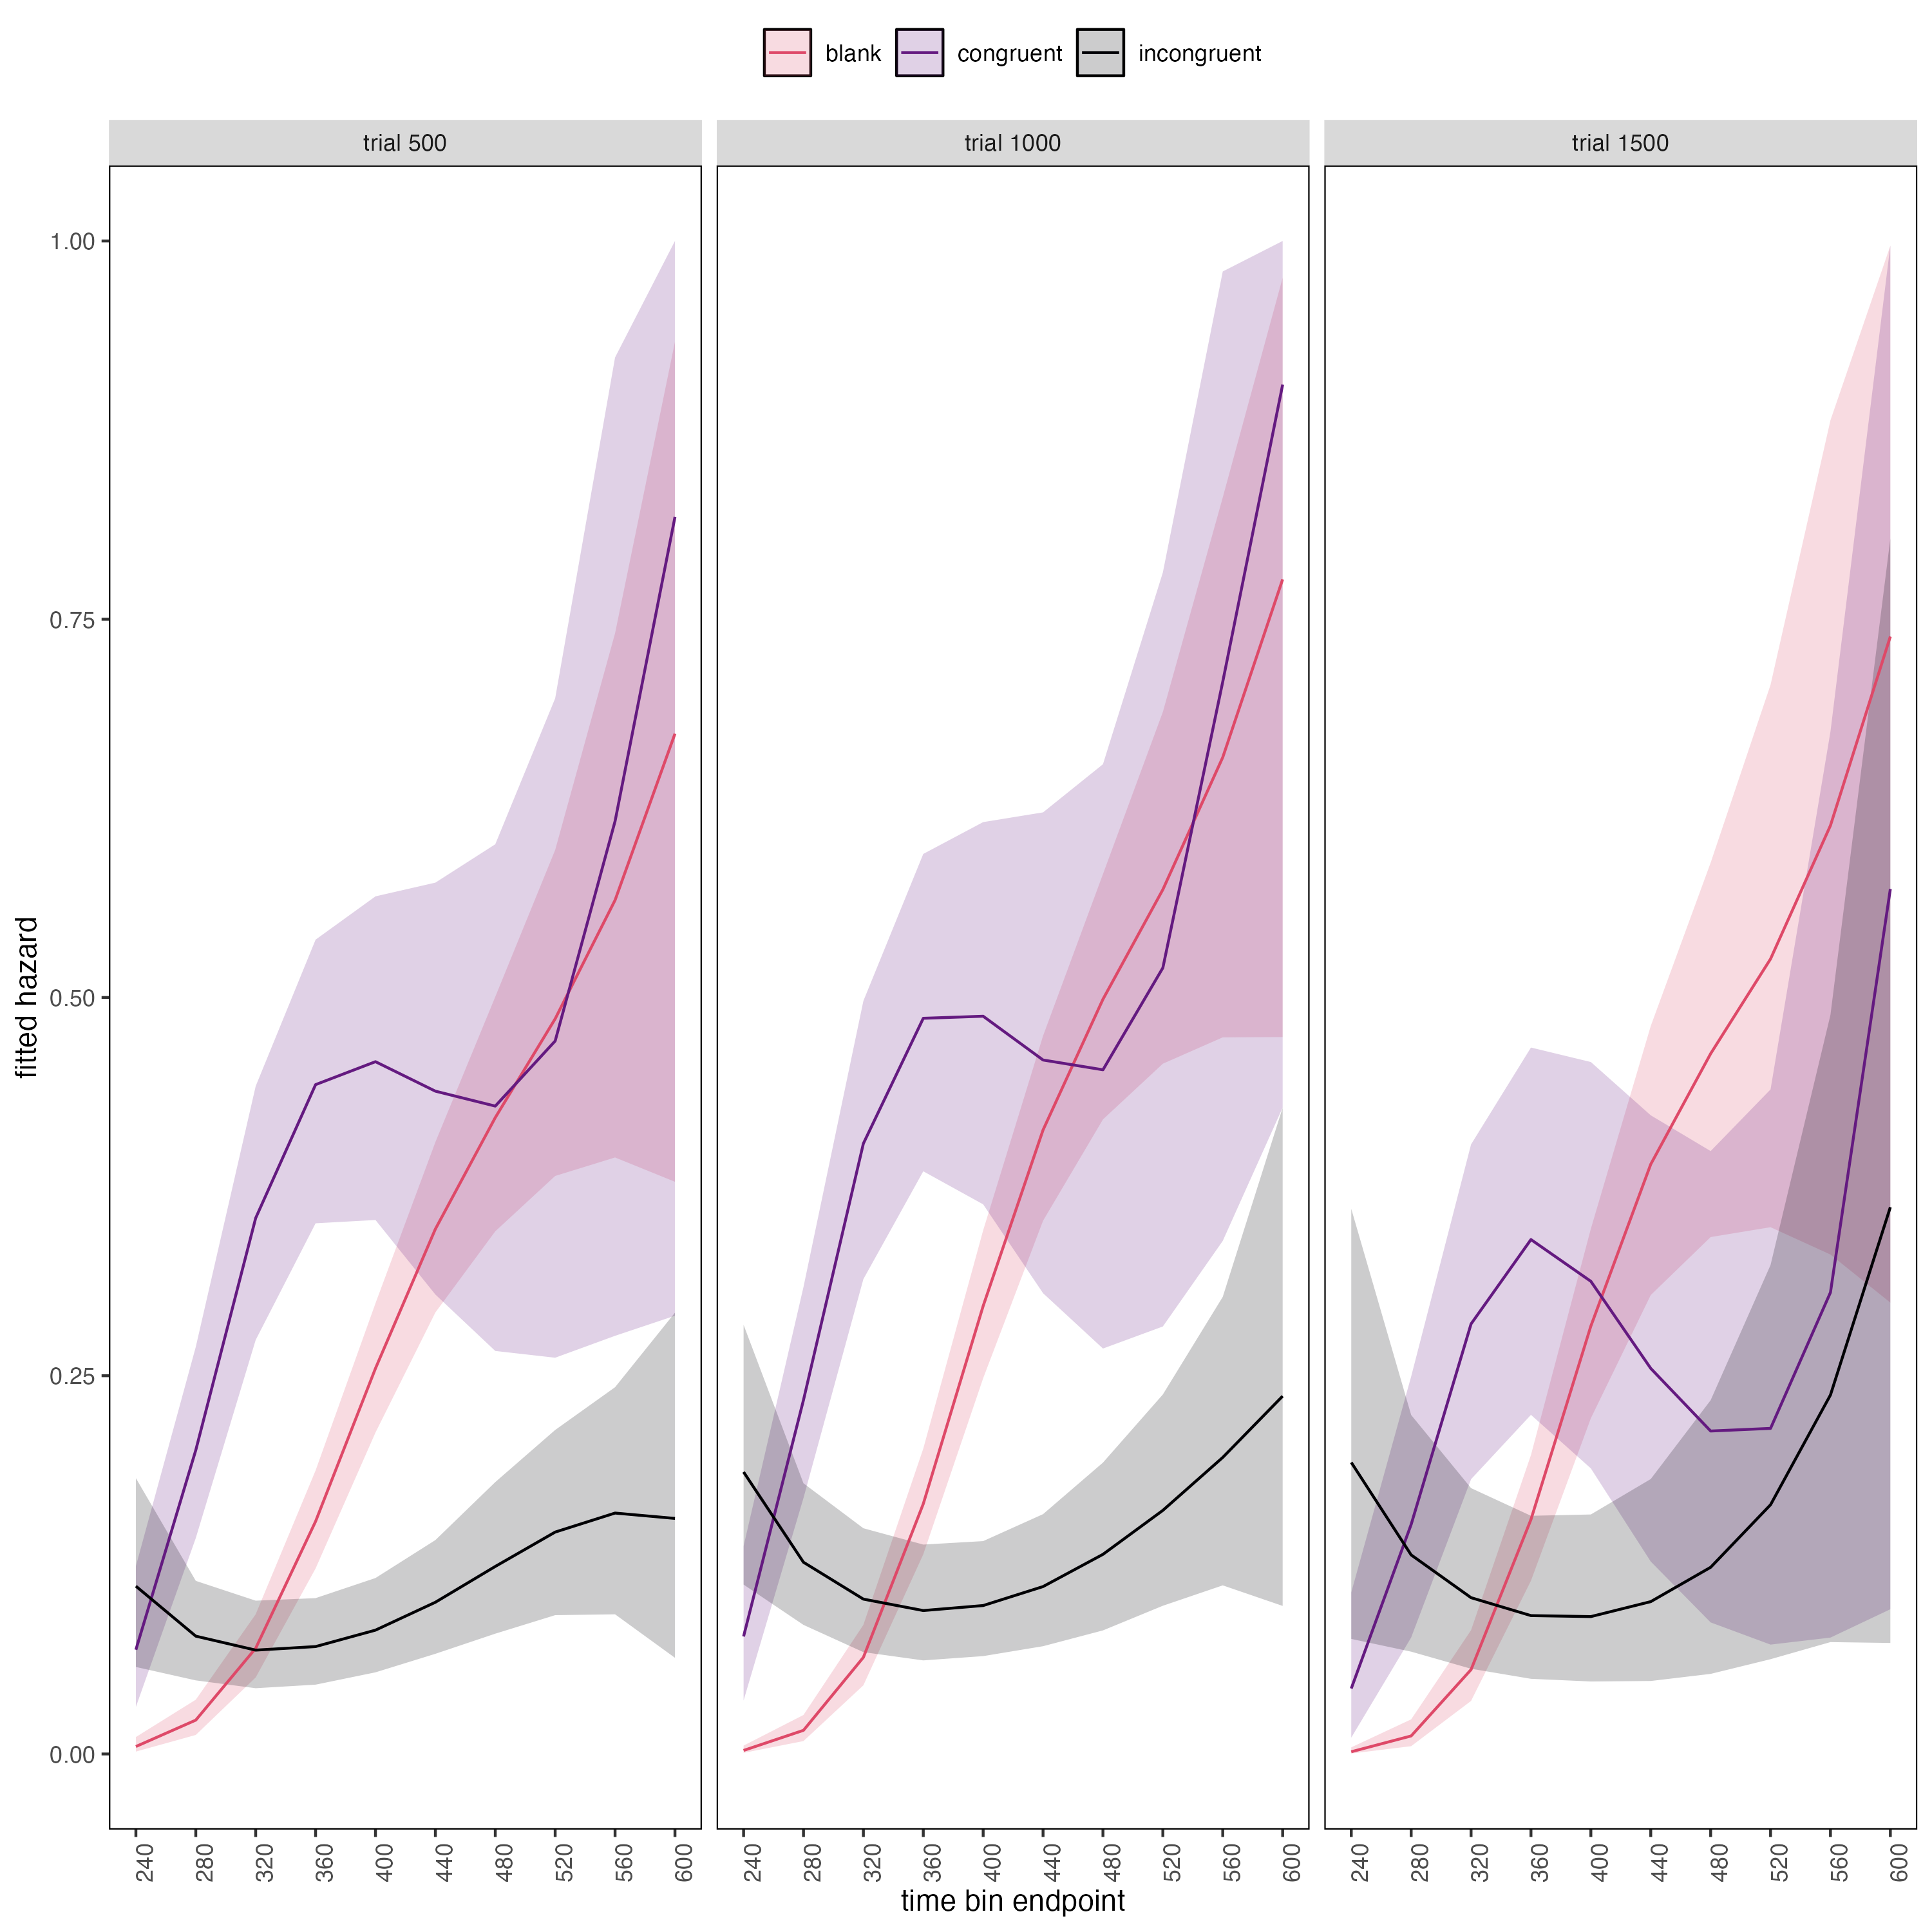
\includegraphics[width=0.8\linewidth,height=0.67\textheight,]{../Tutorial_2_Bayesian/figures/M4effects_subject6} 

}

\caption{Model-based hazard functions for participant 6 in trial 500, 1000, and 1500.}\label{fig:plot-hazard-subject6}
\end{figure}

{[}{[}let's have a paragraph on how we might interpret these plots.{]}{]}

\subsection{4.4 Tutorial 2b: Fitting Bayesian conditional accuracy models}\label{tutorial-2b-fitting-bayesian-conditional-accuracy-models}

\subsection{4.5 Tutorial 3a: Fitting Frequentist hazard models}\label{tutorial-3a-fitting-frequentist-hazard-models}

In this third tutorial we illustrate how to fit a multilevel hazard regression model in the frequentist framework, for the data set used in the first tutorial. For illustration purposes, we only fitted model M3 using the function glmer() from the package lme4.

In Figure 7 we compare the parameter estimates of model M3 from brm() with those of glmer().



\begin{figure}[H]

{\centering \includegraphics[width=0.8\linewidth,height=0.67\textheight,]{../Tutorial_3_Frequentist/comparison} 

}

\caption{Parameter estimates for model M3 from brm() and glmer().}\label{fig:plot-comparison}
\end{figure}

Figure 7 confirms that the parameter estimates from both Bayesian and frequentist models are pretty similar. However, the random effects structure of model M3 was already too complex for the frequentist model as it did not converge and resulted in a singular fit. This is of course one of the reasons why Bayesian modeling has become so popular in recent years. But the price you pay for being able to fit more complex models in a Bayesian framework is computation time. In other words, as we have noted throughout, some of the Bayesian models in Tutorial 2 took several hours to build.

\subsection{4.6 Tutorial 3b: Fitting Frequentist conditional accuracy models}\label{tutorial-3b-fitting-frequentist-conditional-accuracy-models}

\section{5. Discussion}\label{discussion}

This main motivation for writing this paper is the observation that event history analysis remains under-used in psychological research, which means the field of research is not taking full advantage of the many benefits EHA provides compared to more conventional analyses. By providing a freely available set of tutorials, which provide step-by-step guidelines and ready-to-use R code, we hope that researchers will feel more comfortable using EHA in the future. Indeed, we hope that our tutorials may help to overcome a barrier to entry with EHA, which is the increase in analytical complexity compared to mean-average comparisons. While we have focused here on within-subject, factorial, small-\emph{N} designs, it is important to realize that event history analysis can be applied to other designs as well (large-\emph{N} designs with only one measurement per subject, between-subject designs, etc.). As such, the general workflow and associated code can be modified and applied more broadly to other contexts and research questions. In the following, we discuss issues relating to individual differences, limitations of the approach, and future extensions.

\subsection{5.1 Advantages of hazard analysis}\label{advantages-of-hazard-analysis}

Statisticians and mathematical psychologists recommend focusing on the hazard function when analyzing time-to-event data for various reasons. First, as discussed by Holden, Van Orden, and Turvey (2009), ``probability density functions can appear nearly identical, both statistically and to the naked eye, and yet are clearly different on the basis of their hazard functions (but not vice versa). Hazard functions are thus more diagnostic than density functions'' (p.~331) when one is interested in studying the detailed shape of a RT distribution (see also Figure 1 in Panis, Schmidt, et al., 2020). Therefore, {[}{[}why should people care? What is the functional relevance for exp psych and researchers?{]}{]}

{[}{[}This para needs to be way shorter and easier to read or we get rid of it{]}{]}
Second, because RT distributions may differ from one another in multiple ways, Townsend (1990) developed a dominance hierarchy of statistical differences between two arbitrary distributions A and B. For example, if F\textsubscript{A}(t) \textgreater{} F\textsubscript{B}(t) for all t, then both cumulative distribution functions are said to show a complete ordering. Townsend (1990) showed that a complete ordering on the hazard functions ---\(\lambda\)\textsubscript{A}(t) \textgreater{} \(\lambda\)\textsubscript{B}(t) for all t--- implies a complete ordering on both the cumulative distribution and survivor functions ---F\textsubscript{A}(t) \textgreater{} F\textsubscript{B}(t) and S\textsubscript{A}(t) \textless{} S\textsubscript{B}(t)--- which in turn implies an ordering on the mean latencies ---mean A \textless{} mean B. In contrast, an ordering on two means does \emph{not} imply a complete ordering on the corresponding F(t) and S(t) functions, and a complete ordering on these latter functions does \emph{not} imply a complete ordering on the corresponding hazard functions. This means that stronger conclusions can be drawn from data when comparing the hazard functions using EHA. For example, when mean A \textless{} mean B, the hazard functions might show a complete ordering (i.e., for all t), a partial ordering (e.g., only for t \textgreater{} 300 ms, or only for t \textless{} 500 ms), or they may cross each other one or more times.
As a result, instead of using delta-plots for RT -- differences in quantiles from F(t)\(^-1\) -- one can simply plot delta-h(t) functions (see Panis, 2020).

Third, EHA does not discard right-censored observations when estimating hazard functions, that is, trials for which we do not observe a response during the data collection period in a trial so that we only know that the RT must be larger than some value (i.e., the response deadline). This is important because although a few right-censored observations are inevitable in most RT tasks, a lot of right-censored observations are expected in experiments on masking, the attentional blink, and so forth. In other words, by using EHA you can analyze RT data from experiments that typically do not measure response times. As a result, EHA can also deal with long RTs in experiments without a response deadline, which are typically treated as outliers and are discarded before calculating a mean. This orthodox procedure can lead to a sampling bias, however, which results in underestimation of the mean. By introducting a fixed censoring time for all trials at the end of the analysis time window, trials with long RTs are not discarded but contribute to the risk set of each bin.

Fourth, hazard modeling allows incorporating time-varying explanatory covariates such as heart rate, electroencephalogram (EEG) signal amplitude, gaze location, etc. (Allison, 2010). This is useful for linking physiological effects with behavioral effeccts when performing cognitive psychophysiology (Meyer, Osman, Irwin, \& Yantis, 1988).

Finally, as explained by Kelso, Dumas, and Tognoli (2013), it is crucial to first have a precise description of the macroscopic behavior of a system (here: h(t) and ca(t) functions) in order to know what to derive on the microscopic level. EHA can thus solve the problem of model mimicry, i.e., the fact that different computational models can often predict the same mean RTs as observed in the empirical data, but not necessarily the detailed shapes of the empirical RT hazard distributions. Also, fitting parametric functions or computational models to data without studying the shape of the empirical discrete-time h(t) and ca(t) functions can miss important features in the data (Panis, Moran, et al., 2020; Panis \& Schmidt, 2016).

\subsection{5.2 Individual differences}\label{individual-differences}

One important issue is that of possible individual differences in the overall location of the distribution, and the time course of psychological effects. For example, when you wait for a response of the participant on each trial, you allow the participant to have control over the trial duration, and some participants might respond only when they are confident that their emitted response will be correct. These issues can be avoided by introducing a (relatively short) response deadline in each trial, e.g., 600 ms for simple detection tasks, 1000 ms for more difficult discrimination tasks, or 2 s for tasks requiring extended high-level processing. Because EHA can deal in a straightforward fashion with right-censored observations (i.e., trials without an observed response), introducing a response deadline is recommended when designing RT experiments. Furthermore, introducing a response deadline and asking participants to respond before the deadline as much as possible, will also lead to individual distributions that overlap in time, which is important when selecting a common analysis time window when fitting hazard models.

But even when using a response deadline, participants can differ qualitatively in the effects they display (see Panis, 2020). One way to deal with this is to describe and interpret the different patterns. Another way is to run a clustering algorithm on the individual hazard estimates across all conditions. The obtained dendrogram can then be used to identify a (hopefully big) cluster of participants that behave similarly, and to identify a (hopefully small) cluster of participants with outlying behavioral patterns. One might then exclude the outlying participants before fitting a hazard model.

\subsection{5.3 Limitation(s)}\label{limitations}

Compared to the orthodox method -- comparing mean-averages between conditions -- the most important limitation of multilevel hazard modeling is that it might take a long time to estimate the parameters using Bayesian methods or the model might have to be simplified significantly to use frequentist methods.

Another issue is that you need a relatively large number of trials per condition to estimate the hazard function with high temporal resolution. Indeed, in general, there is a trade-off between the number of trials per condition and the temporal resolution (i.e., bin width) of the hazard function. Therefore, we recommend researchers to collect as many trials as possible per experimental condition, given the available resources and considering the participant experience (e.g., fatigue and boredom). For instance, if the maximum session length deemed reasonable is between 1 and 2 hours, what is the maximum number of trials per condition that you could reasonably collect? After consideration, it might be worth conducting multiple testing sessions per participant and/or reducing the number of experimental conditions. Finally, there is a user-friendly online tool for calculating statistical power as a function of the number of trials as well as the number of participants, and this might be worth consulting to guide the research design process (Baker et al., 2021).

We did not discuss continuous-time hazard analysis. As indicated by --allison -- learning discrete-time methods first will help in learning continuous-time methods. Given that RT is typically treated as a continuous variable, it is possible that continuous-time methods will ultimately prevail. However, they require much more data to estimate the continuous-time hazard (rate) function well. Thus, by trading a bit of temporal resolution for a lower number of trials, discrete-time methods seem ideal for dealing with typical psychological time-to-event data sets for which there are less than \textasciitilde200 trials per condition per experiment.

\subsection{5.4 Extensions}\label{extensions}

The hazard models in this tutorial assume that there is one event of interest. For RT data, this event constitutes a single transition between an ``idle'' state and a ``responded'' state. However, in certain situations, more than one event of interest might exist. For example, in a medical or health-related context, an individual might transition back and forth between a ``healthy'' state and a ``depressed'' state, before a final ``death'' state. When you have data on the timing of these transitions, one can apply multi-state models, which generalize survival analysis to transitions between three or more states (Steele, Goldstein, \& Browne, 2004).
Also, the predictor variables in this tutorial are time-invariant, i.e., their value did not change over the course of a trial. Thus, another extension is to include time-varying predictors, i.e., predictors whose value can change across the time bins within a trial (REF). {[}{[}give a concrete example for this latter point{]}{]}

\section{6. Conclusions}\label{conclusions}

RT and accuracy distributions are a rich source of information on the time course of cognitive processing, which have been largely undervalued in the history of experimental psychology and cognitive neuroscience. We hope that by providing a set of hands-on, step-by-step tutorials, which come with custom-built and freely available code, researchers will feel more comfortable embracing event history analysis and investigating the temporal profile of cognitive states. On a broader level, we think that wider adoption of such approaches will have a meaningful impact on the inferences drawn from data, as well as the development of theories regarding the structure of cognition.

\newpage

\section{References}\label{references}

\phantomsection\label{refs}
\begin{CSLReferences}{1}{0}
\bibitem[\citeproctext]{ref-allisonDiscreteTimeMethodsAnalysis1982}
Allison, P. D. (1982). Discrete-{Time Methods} for the {Analysis} of {Event Histories}. \emph{Sociological Methodology}, \emph{13}, 61. \url{https://doi.org/10.2307/270718}

\bibitem[\citeproctext]{ref-allisonSurvivalAnalysisUsing2010}
Allison, P. D. (2010). \emph{Survival analysis using {SAS}: A practical guide} (2. ed). Cary, NC: SAS Press.

\bibitem[\citeproctext]{ref-R-citr}
Aust, F. (2019). \emph{Citr: 'RStudio' add-in to insert markdown citations}. Retrieved from \url{https://github.com/crsh/citr}

\bibitem[\citeproctext]{ref-R-papaja}
Aust, F., \& Barth, M. (2023). \emph{{papaja}: {Prepare} reproducible {APA} journal articles with {R Markdown}}. Retrieved from \url{https://github.com/crsh/papaja}

\bibitem[\citeproctext]{ref-bakerPowerContoursOptimising2021}
Baker, D. H., Vilidaite, G., Lygo, F. A., Smith, A. K., Flack, T. R., Gouws, A. D., \& Andrews, T. J. (2021). Power contours: {Optimising} sample size and precision in experimental psychology and human neuroscience. \emph{Psychological Methods}, \emph{26}(3), 295--314. \url{https://doi.org/10.1037/met0000337}

\bibitem[\citeproctext]{ref-R-tinylabels}
Barth, M. (2023). \emph{{tinylabels}: Lightweight variable labels}. Retrieved from \url{https://cran.r-project.org/package=tinylabels}

\bibitem[\citeproctext]{ref-R-lme4}
Bates, D., Mächler, M., Bolker, B., \& Walker, S. (2015). Fitting linear mixed-effects models using {lme4}. \emph{Journal of Statistical Software}, \emph{67}(1), 1--48. \url{https://doi.org/10.18637/jss.v067.i01}

\bibitem[\citeproctext]{ref-R-Matrix}
Bates, D., Maechler, M., \& Jagan, M. (2024). \emph{Matrix: Sparse and dense matrix classes and methods}. Retrieved from \url{https://CRAN.R-project.org/package=Matrix}

\bibitem[\citeproctext]{ref-R-RJ-2021-048}
Bengtsson, H. (2021). A unifying framework for parallel and distributed processing in r using futures. \emph{The R Journal}, \emph{13}(2), 208--227. \url{https://doi.org/10.32614/RJ-2021-048}

\bibitem[\citeproctext]{ref-R-brms_a}
Bürkner, P.-C. (2017). {brms}: An {R} package for {Bayesian} multilevel models using {Stan}. \emph{Journal of Statistical Software}, \emph{80}(1), 1--28. \url{https://doi.org/10.18637/jss.v080.i01}

\bibitem[\citeproctext]{ref-R-brms_b}
Bürkner, P.-C. (2018). Advanced {Bayesian} multilevel modeling with the {R} package {brms}. \emph{The R Journal}, \emph{10}(1), 395--411. \url{https://doi.org/10.32614/RJ-2018-017}

\bibitem[\citeproctext]{ref-R-brms_c}
Bürkner, P.-C. (2021). Bayesian item response modeling in {R} with {brms} and {Stan}. \emph{Journal of Statistical Software}, \emph{100}(5), 1--54. \url{https://doi.org/10.18637/jss.v100.i05}

\bibitem[\citeproctext]{ref-R-Rcpp_b}
Eddelbuettel, D., \& Balamuta, J. J. (2018). {Extending {R} with {C++}: A Brief Introduction to {Rcpp}}. \emph{The American Statistician}, \emph{72}(1), 28--36. \url{https://doi.org/10.1080/00031305.2017.1375990}

\bibitem[\citeproctext]{ref-R-Rcpp_a}
Eddelbuettel, D., \& François, R. (2011). {Rcpp}: Seamless {R} and {C++} integration. \emph{Journal of Statistical Software}, \emph{40}(8), 1--18. \url{https://doi.org/10.18637/jss.v040.i08}

\bibitem[\citeproctext]{ref-R-cmdstanr}
Gabry, J., Češnovar, R., Johnson, A., \& Bronder, S. (2024). \emph{Cmdstanr: R interface to 'CmdStan'}. Retrieved from \url{https://github.com/stan-dev/cmdstanr}

\bibitem[\citeproctext]{ref-R-bayesplot}
Gabry, J., Simpson, D., Vehtari, A., Betancourt, M., \& Gelman, A. (2019). Visualization in bayesian workflow. \emph{J. R. Stat. Soc. A}, \emph{182}, 389--402. \url{https://doi.org/10.1111/rssa.12378}

\bibitem[\citeproctext]{ref-R-standist}
Girard, J. (2024). \emph{Standist: What the package does (one line, title case)}. Retrieved from \url{https://github.com/jmgirard/standist}

\bibitem[\citeproctext]{ref-R-lubridate}
Grolemund, G., \& Wickham, H. (2011). Dates and times made easy with {lubridate}. \emph{Journal of Statistical Software}, \emph{40}(3), 1--25. Retrieved from \url{https://www.jstatsoft.org/v40/i03/}

\bibitem[\citeproctext]{ref-holdenDispersionResponseTimes2009}
Holden, J. G., Van Orden, G. C., \& Turvey, M. T. (2009). Dispersion of response times reveals cognitive dynamics. \emph{Psychological Review}, \emph{116}(2), 318--342. \url{https://doi.org/10.1037/a0014849}

\bibitem[\citeproctext]{ref-kantowitzInterpretationReactionTime2021}
Kantowitz, B. H., \& Pachella, R. G. (2021). The {Interpretation} of {Reaction Time} in {Information-Processing Research} 1. \emph{Human Information Processing}, 41--82. \url{https://doi.org/10.4324/9781003176688-2}

\bibitem[\citeproctext]{ref-R-tidybayes}
Kay, M. (2023). \emph{{tidybayes}: Tidy data and geoms for {Bayesian} models}. \url{https://doi.org/10.5281/zenodo.1308151}

\bibitem[\citeproctext]{ref-kelsoOutlineGeneralTheory2013}
Kelso, J. A. S., Dumas, G., \& Tognoli, E. (2013). Outline of a general theory of behavior and brain coordination. \emph{Neural Networks: The Official Journal of the International Neural Network Society}, \emph{37}, 120--131. \url{https://doi.org/10.1016/j.neunet.2012.09.003}

\bibitem[\citeproctext]{ref-kurzAppliedLongitudinalDataAnalysis2023}
Kurz, A. S. (2023a). \emph{Applied longitudinal data analysis in brms and the tidyverse} (version 0.0.3). Retrieved from \url{https://bookdown.org/content/4253/}

\bibitem[\citeproctext]{ref-kurzStatisticalRethinkingSecondEd2023}
Kurz, A. S. (2023b). \emph{Statistical rethinking with brms, ggplot2, and the tidyverse: {Second} edition} (version 0.4.0). Retrieved from \url{https://bookdown.org/content/4857/}

\bibitem[\citeproctext]{ref-luceResponseTimesTheir1991}
Luce, R. D. (1991). \emph{Response times: Their role in inferring elementary mental organization} (1. issued as paperback). Oxford: Univ. Press.

\bibitem[\citeproctext]{ref-mcelreathStatisticalRethinkingBayesian2018}
McElreath, R. (2018). \emph{Statistical {Rethinking}: {A Bayesian Course} with {Examples} in {R} and {Stan}} (1st ed.). {Chapman and Hall/CRC}. \url{https://doi.org/10.1201/9781315372495}

\bibitem[\citeproctext]{ref-meyerModernMentalChronometry1988}
Meyer, D. E., Osman, A. M., Irwin, D. E., \& Yantis, S. (1988). Modern mental chronometry. \emph{Biological Psychology}, \emph{26}(1-3), 3--67. \url{https://doi.org/10.1016/0301-0511(88)90013-0}

\bibitem[\citeproctext]{ref-R-tibble}
Müller, K., \& Wickham, H. (2023). \emph{Tibble: Simple data frames}. Retrieved from \url{https://CRAN.R-project.org/package=tibble}

\bibitem[\citeproctext]{ref-R-RColorBrewer}
Neuwirth, E. (2022). \emph{RColorBrewer: ColorBrewer palettes}. Retrieved from \url{https://CRAN.R-project.org/package=RColorBrewer}

\bibitem[\citeproctext]{ref-panisHowCanWe2020}
Panis, S. (2020). How can we learn what attention is? {Response} gating via multiple direct routes kept in check by inhibitory control processes. \emph{Open Psychology}, \emph{2}(1), 238--279. \url{https://doi.org/10.1515/psych-2020-0107}

\bibitem[\citeproctext]{ref-panisStudyingDynamicsVisual2020}
Panis, S., Moran, R., Wolkersdorfer, M. P., \& Schmidt, T. (2020). Studying the dynamics of visual search behavior using {RT} hazard and micro-level speed--accuracy tradeoff functions: {A} role for recurrent object recognition and cognitive control processes. \emph{Attention, Perception, \& Psychophysics}, \emph{82}(2), 689--714. \url{https://doi.org/10.3758/s13414-019-01897-z}

\bibitem[\citeproctext]{ref-panisAnalyzingResponseTimes2020}
Panis, S., Schmidt, F., Wolkersdorfer, M. P., \& Schmidt, T. (2020). Analyzing {Response Times} and {Other Types} of {Time-to-Event Data Using Event History Analysis}: {A Tool} for {Mental Chronometry} and {Cognitive Psychophysiology}. \emph{I-Perception}, \emph{11}(6), 2041669520978673. \url{https://doi.org/10.1177/2041669520978673}

\bibitem[\citeproctext]{ref-panisWhatShapingRT2016}
Panis, S., \& Schmidt, T. (2016). What {Is Shaping RT} and {Accuracy Distributions}? {Active} and {Selective Response Inhibition Causes} the {Negative Compatibility Effect}. \emph{Journal of Cognitive Neuroscience}, \emph{28}(11), 1651--1671. \url{https://doi.org/10.1162/jocn_a_00998}

\bibitem[\citeproctext]{ref-panisWhenDoesInhibition2022}
Panis, S., \& Schmidt, T. (2022). When does {``inhibition of return''} occur in spatial cueing tasks? {Temporally} disentangling multiple cue-triggered effects using response history and conditional accuracy analyses. \emph{Open Psychology}, \emph{4}(1), 84--114. \url{https://doi.org/10.1515/psych-2022-0005}

\bibitem[\citeproctext]{ref-panisNeuropsychologicalEvidenceTemporal2017}
Panis, S., Torfs, K., Gillebert, C. R., Wagemans, J., \& Humphreys, G. W. (2017). Neuropsychological evidence for the temporal dynamics of category-specific naming. \emph{Visual Cognition}, \emph{25}(1-3), 79--99. \url{https://doi.org/10.1080/13506285.2017.1330790}

\bibitem[\citeproctext]{ref-panisTimecourseContingenciesPerceptual2009}
Panis, S., \& Wagemans, J. (2009). Time-course contingencies in perceptual organization and identification of fragmented object outlines. \emph{Journal of Experimental Psychology: Human Perception and Performance}, \emph{35}(3), 661--687. \url{https://doi.org/10.1037/a0013547}

\bibitem[\citeproctext]{ref-R-patchwork}
Pedersen, T. L. (2024). \emph{Patchwork: The composer of plots}. Retrieved from \url{https://CRAN.R-project.org/package=patchwork}

\bibitem[\citeproctext]{ref-R-nlme}
Pinheiro, J. C., \& Bates, D. M. (2000). \emph{Mixed-effects models in s and s-PLUS}. New York: Springer. \url{https://doi.org/10.1007/b98882}

\bibitem[\citeproctext]{ref-R-base}
R Core Team. (2024). \emph{R: A language and environment for statistical computing}. Vienna, Austria: R Foundation for Statistical Computing. Retrieved from \url{https://www.R-project.org/}

\bibitem[\citeproctext]{ref-singerAppliedLongitudinalData2003}
Singer, J. D., \& Willett, J. B. (2003). \emph{Applied {Longitudinal Data Analysis}: {Modeling Change} and {Event Occurrence}}. Oxford, New York: Oxford University Press.

\bibitem[\citeproctext]{ref-smithSmallBeautifulDefense2018}
Smith, P. L., \& Little, D. R. (2018). Small is beautiful: {In} defense of the small-{N} design. \emph{Psychonomic Bulletin \& Review}, \emph{25}(6), 2083--2101. \url{https://doi.org/10.3758/s13423-018-1451-8}

\bibitem[\citeproctext]{ref-SteeleF2004}
Steele, F., Goldstein, H., \& Browne, W. (2004). A general multilevel multistate competing risks model for event history data, with an application to a study of contraceptive use dynamics. \emph{Statistical Modelling}, \emph{4}(2), 145--159. \url{https://doi.org/10.1191/1471082X04st069oa}

\bibitem[\citeproctext]{ref-townsendTruthConsequencesOrdinal1990}
Townsend, J. T. (1990). Truth and consequences of ordinal differences in statistical distributions: {Toward} a theory of hierarchical inference. \emph{Psychological Bulletin}, \emph{108}(3), 551--567. \url{https://doi.org/10.1037/0033-2909.108.3.551}

\bibitem[\citeproctext]{ref-wickelgrenSpeedaccuracyTradeoffInformation1977}
Wickelgren, W. A. (1977). Speed-accuracy tradeoff and information processing dynamics. \emph{Acta Psychologica}, \emph{41}(1), 67--85. \url{https://doi.org/10.1016/0001-6918(77)90012-9}

\bibitem[\citeproctext]{ref-R-ggplot2}
Wickham, H. (2016). \emph{ggplot2: Elegant graphics for data analysis}. Springer-Verlag New York. Retrieved from \url{https://ggplot2.tidyverse.org}

\bibitem[\citeproctext]{ref-R-forcats}
Wickham, H. (2023a). \emph{Forcats: Tools for working with categorical variables (factors)}. Retrieved from \url{https://forcats.tidyverse.org/}

\bibitem[\citeproctext]{ref-R-stringr}
Wickham, H. (2023b). \emph{Stringr: Simple, consistent wrappers for common string operations}. Retrieved from \url{https://stringr.tidyverse.org}

\bibitem[\citeproctext]{ref-R-tidyverse}
Wickham, H., Averick, M., Bryan, J., Chang, W., McGowan, L. D., François, R., \ldots{} Yutani, H. (2019). Welcome to the {tidyverse}. \emph{Journal of Open Source Software}, \emph{4}(43), 1686. \url{https://doi.org/10.21105/joss.01686}

\bibitem[\citeproctext]{ref-R-dplyr}
Wickham, H., François, R., Henry, L., Müller, K., \& Vaughan, D. (2023). \emph{Dplyr: A grammar of data manipulation}. Retrieved from \url{https://dplyr.tidyverse.org}

\bibitem[\citeproctext]{ref-R-purrr}
Wickham, H., \& Henry, L. (2023). \emph{Purrr: Functional programming tools}. Retrieved from \url{https://purrr.tidyverse.org/}

\bibitem[\citeproctext]{ref-R-readr}
Wickham, H., Hester, J., \& Bryan, J. (2024). \emph{Readr: Read rectangular text data}. Retrieved from \url{https://readr.tidyverse.org}

\bibitem[\citeproctext]{ref-R-tidyr}
Wickham, H., Vaughan, D., \& Girlich, M. (2024). \emph{Tidyr: Tidy messy data}. Retrieved from \url{https://tidyr.tidyverse.org}

\end{CSLReferences}

\newpage

\section{Supplementary material}\label{supplementary-material}

\subsection{A. Definitions of discrete-time hazard, surivor, and conditional accuracy functions}\label{a.-definitions-of-discrete-time-hazard-surivor-and-conditional-accuracy-functions}

The shape of a distribution of waiting times can be described in multiple ways (Luce, 1991). After dividing time in discrete, contiguous time bins indexed by t, let RT be a discrete random variable denoting the rank of the time bin in which a particular person's response occurs in a particular experimental condition.
Discrete-time EHA focuses on the discrete-time hazard function

\noindent h(t) = P(RT = t\textbar{} RT \(\geq\) t) \hfill  (1)

\noindent and the discrete-time survivor function

\noindent S(t) = P(RT \(>\) t) = {[}1-h(t){]}.{[}1-h(t-1){]}.{[}1-h(t-2){]}\ldots{[}1-h(1){]} \hfill  (2)

\noindent and not on the probability mass function

\noindent P(t) = P(RT = t) = h(t).S(t-1) \hfill  (3)

\noindent nor the cumulative distribution function

\noindent F(t) = P(RT \(\leq\) t) = 1-S(t) \hfill  (4)

The discrete-time hazard function of event occurrence gives you the probability that the event occurs (sometime) in bin t, given that the event has not occurred yet in previous bins. While the discrete-time hazard function assesses the unique risk of event occurrence associated with each time bin, the discrete-time survivor function cumulates the bin-by-bin risks of event \emph{non}occurrence to obtain the probability that the event occurs afer bin t. The probability mass function cumulates the risk of event occurrence in bin t with the risks of event nonoccurrence in bins 1 to t-1. From equation 3 we find that hazard in bin t is equal to P(t)/S(t-1).

For two-choice RT data, the discrete-time hazard function can be extended with the discrete-time conditional accuracy function

\noindent ca(t) = P(correct \textbar{} RT = t) \hfill  (5)

which gives you the probability that a response is correct given that it is emitted in time bin t (Allison, 2010; Kantowitz \& Pachella, 2021; Wickelgren, 1977). This latter function is also known as the micro-level speed-accuracy tradeoff (SAT) function.

The survivor function provides a context for the hazard function, as S(t-1) = P(RT \textgreater{} t-1) = P(RT \textgreater= t) tells you on how many percent of the trials the estimate h(t) = .. is based. The probability mass function provides a context for the conditional accuracy function, as P(t) tells you on how many percent of the trials the estimate ca(t) is based.

When time is treated as a continuous variable, let RT be a continous random variable denoting a particular person's response time in a particular experimental condition. Because waiting times can only increase, continuous-time EHA does not focus on the cumulative distribution function F(t) = P(RT \(\leq\) t) and its derivative, the probability density function f(t) = F(t)', but on the survivor function S(t) = P(RT \(>\) t) and the hazard rate function \(\lambda\)(t) = f(t)/S(t). The hazard rate function gives you the instantaneous \emph{rate} of event occurrence at time point t, given that the event has not occurred yet.

\subsection{B. Custom functions for descriptive discrete-time hazard analysis}\label{b.-custom-functions-for-descriptive-discrete-time-hazard-analysis}

We defined 13 custom functions that we list here.

\begin{itemize}
\tightlist
\item
  censor(df,timeout,bin\_width) : divide the time segment (0,timeout{]} in bins, identify any right-censored observations, and determine the discrete RT (time bin rank)
\item
  ptb(df) : transform the person-trial data set to the person-trial-bin data set
\item
  setup\_lt(ptb) : set up a life table for each level of 1 independent variable
\item
  setup\_lt\_2IV(ptb) : set up a life table for each combination of levels of 2 independent variables
\item
  calc\_ca(df) : estimate the conditinal accuracies when there is 1 independent variable
\item
  calc\_ca\_2IV(df) : estimate the conditional accuraies when there are 2 independent variables
\item
  join\_lt\_ca(df1,df2) : add the ca(t) estimates to the life tables (1 independent variable)
\item
  join\_lt\_ca\_2IV(df1,df2) : add the ca(t) estimates to the life tables (2 independent variables)
\item
  extract\_median(df) : estimate quantiles S(t).50 (1 independent variable)
\item
  extract\_median\_2IV(df) : estimate quantiles S(t).50 (2 independent variables)
\item
  plot\_eha(df,subj,haz\_yaxis) : create plots of the discrete-time functions (1 independent variable)
\item
  plot\_eha\_2IV(df,subj,haz\_yaxis) : create plots of the discrete-time functions (2 independent variables)
\item
  plot\_eha\_agg(df,subj,haz\_yaxis) : create 1 plot for aggregated data (1 independent variable)
\end{itemize}

\subsection{C. Link functions}\label{c.-link-functions}



\begin{figure}[H]

{\centering 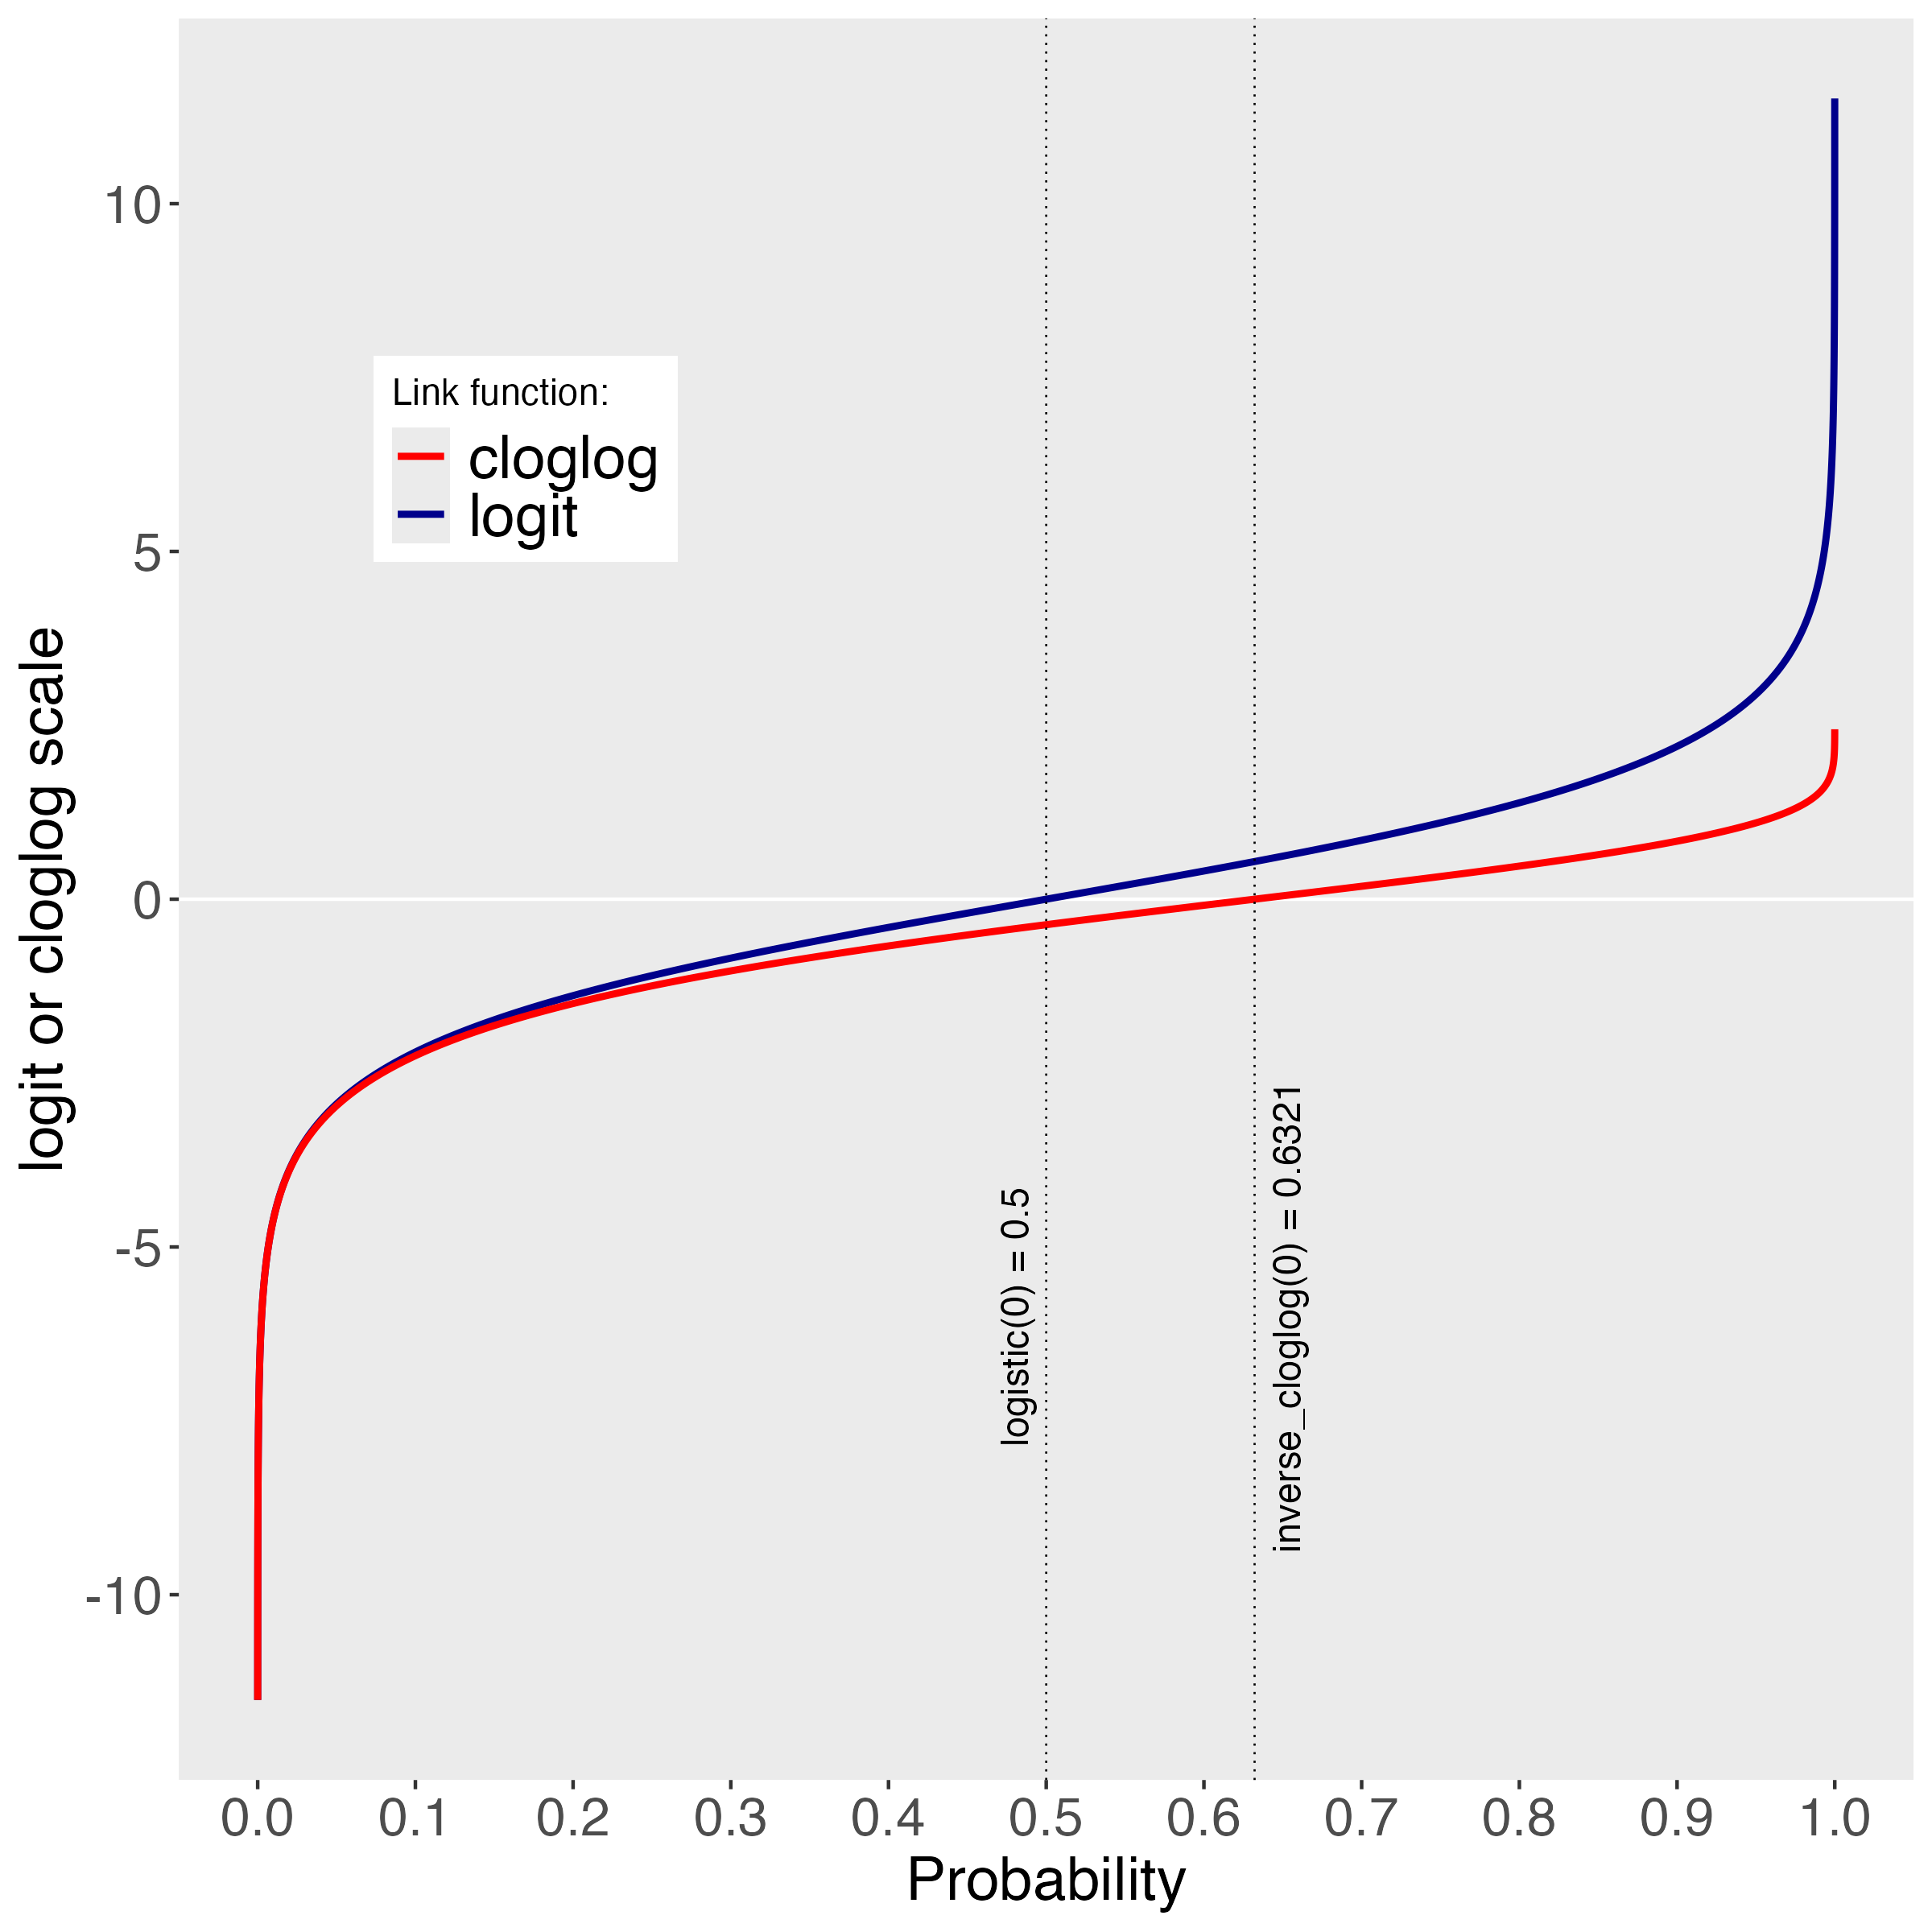
\includegraphics[width=0.8\linewidth,height=0.67\textheight,]{../Tutorial_2_Bayesian/figures/linkfunctions} 

}

\caption{The logit and cloglog link functions.}\label{fig:plot-link-functions}
\end{figure}

\subsection{D. Regression equations}\label{d.-regression-equations}

An example (single-level) discrete-time hazard model with three predictors (TIME, X\textsubscript{1}, X\textsubscript{2}), the cloglog link function, and a third-order polynomial specification for TIME can be written as follows:

cloglog{[}h(t){]} = ln(-ln{[}1-h(t){]}) = {[}\(\alpha\)\textsubscript{1}ONE + \(\alpha\)\textsubscript{2}(TIME-9) + \(\alpha\)\textsubscript{3}(TIME-9)\(^2\){]} + {[}\(\beta\)\textsubscript{1}X\textsubscript{1} + \(\beta\)\textsubscript{2}X\textsubscript{2} + \(\beta\)\textsubscript{3}X\textsubscript{2}(TIME-9){]}

The main predictor variable TIME is the time bin index t that is centered on value 9 in this example. The first set of terms within brackets, the alpha parameters multiplied by their polynomial specifications of (centered) time, represents the shape of the baseline cloglog-hazard function (i.e., when all predictors X\textsubscript{i} take on a value of zero). The second set of terms (the beta parameters) represents the vertical shift in the baseline cloglog-hazard for a 1 unit increase in the respective predictor variable. Predictors can be discrete, continuous, and time-varying or time-invariant. For example, the effect of a 1 unit increase in X\textsubscript{1} is to vertically shift the whole baseline cloglog-hazard function by \(\beta\)\textsubscript{1} cloglog-hazard units. However, if the predictor interacts linearly with TIME (see X\textsubscript{2} in the example), then the effect of a 1 unit increase in X\textsubscript{2} is to vertically shift the predicted cloglog-hazard in bin 9 by \(\beta\)\textsubscript{2} cloglog-hazard units (when TIME-9 = 0), in bin 10 by \(\beta\)\textsubscript{2} + \(\beta\)\textsubscript{3} cloglog-hazard units (when TIME-9 = 1), and so forth. To interpret the effects of a predictor,its \(\beta\) parameter is exponentiated, resulting in a hazard ratio (due to the use of the cloglog link). When using the logit link, exponentiating a \(\beta\) parameter results in an odds ratio.

An example (single-level) discrete-time hazard model with a general specification for TIME (separate intercepts for each of six bins, where D1 to D6 are binary variables identifying each bin) and a single predictor (X\textsubscript{1}) can be written as follows:

cloglog{[}h(t){]} = ln(-ln{[}1-h(t){]}) = {[}\(\alpha\)\textsubscript{1}D1 + \(\alpha\)\textsubscript{2}D2 + \(\alpha\)\textsubscript{3}D3 + \(\alpha\)\textsubscript{4}D4 + \(\alpha\)\textsubscript{5}D5 + \(\alpha\)\textsubscript{6}D6{]} + {[}\(\beta\)\textsubscript{1}X\textsubscript{1}{]}

\subsection{E. Prior distributions}\label{e.-prior-distributions}

To gain a sense of what prior \emph{logit} values would approximate a uniform distribution on the probability scale, Kurz (2023a) simulated a large number of draws from the Uniform(0,1) distribution, converted those draws to the log-odds metric, and fitted a Student's t distribution. Row C in Figure 4 shows that using a t-distribution with 7.61 degrees of freedom and a scale parameter of 1.57 as a prior on the logit scale, approximates a uniform distribution on the probability scale. According to Kurz (2023a), such a prior might be a good prior for the intercept(s) in a logit-hazard model, while the N(0,1) prior in row D might be a good prior for the non-intercept parameters in a logit-hazard model, as it gently regularizes p towards .5 (i.e., a zero effect on the logit scale).



\begin{figure}[H]

{\centering 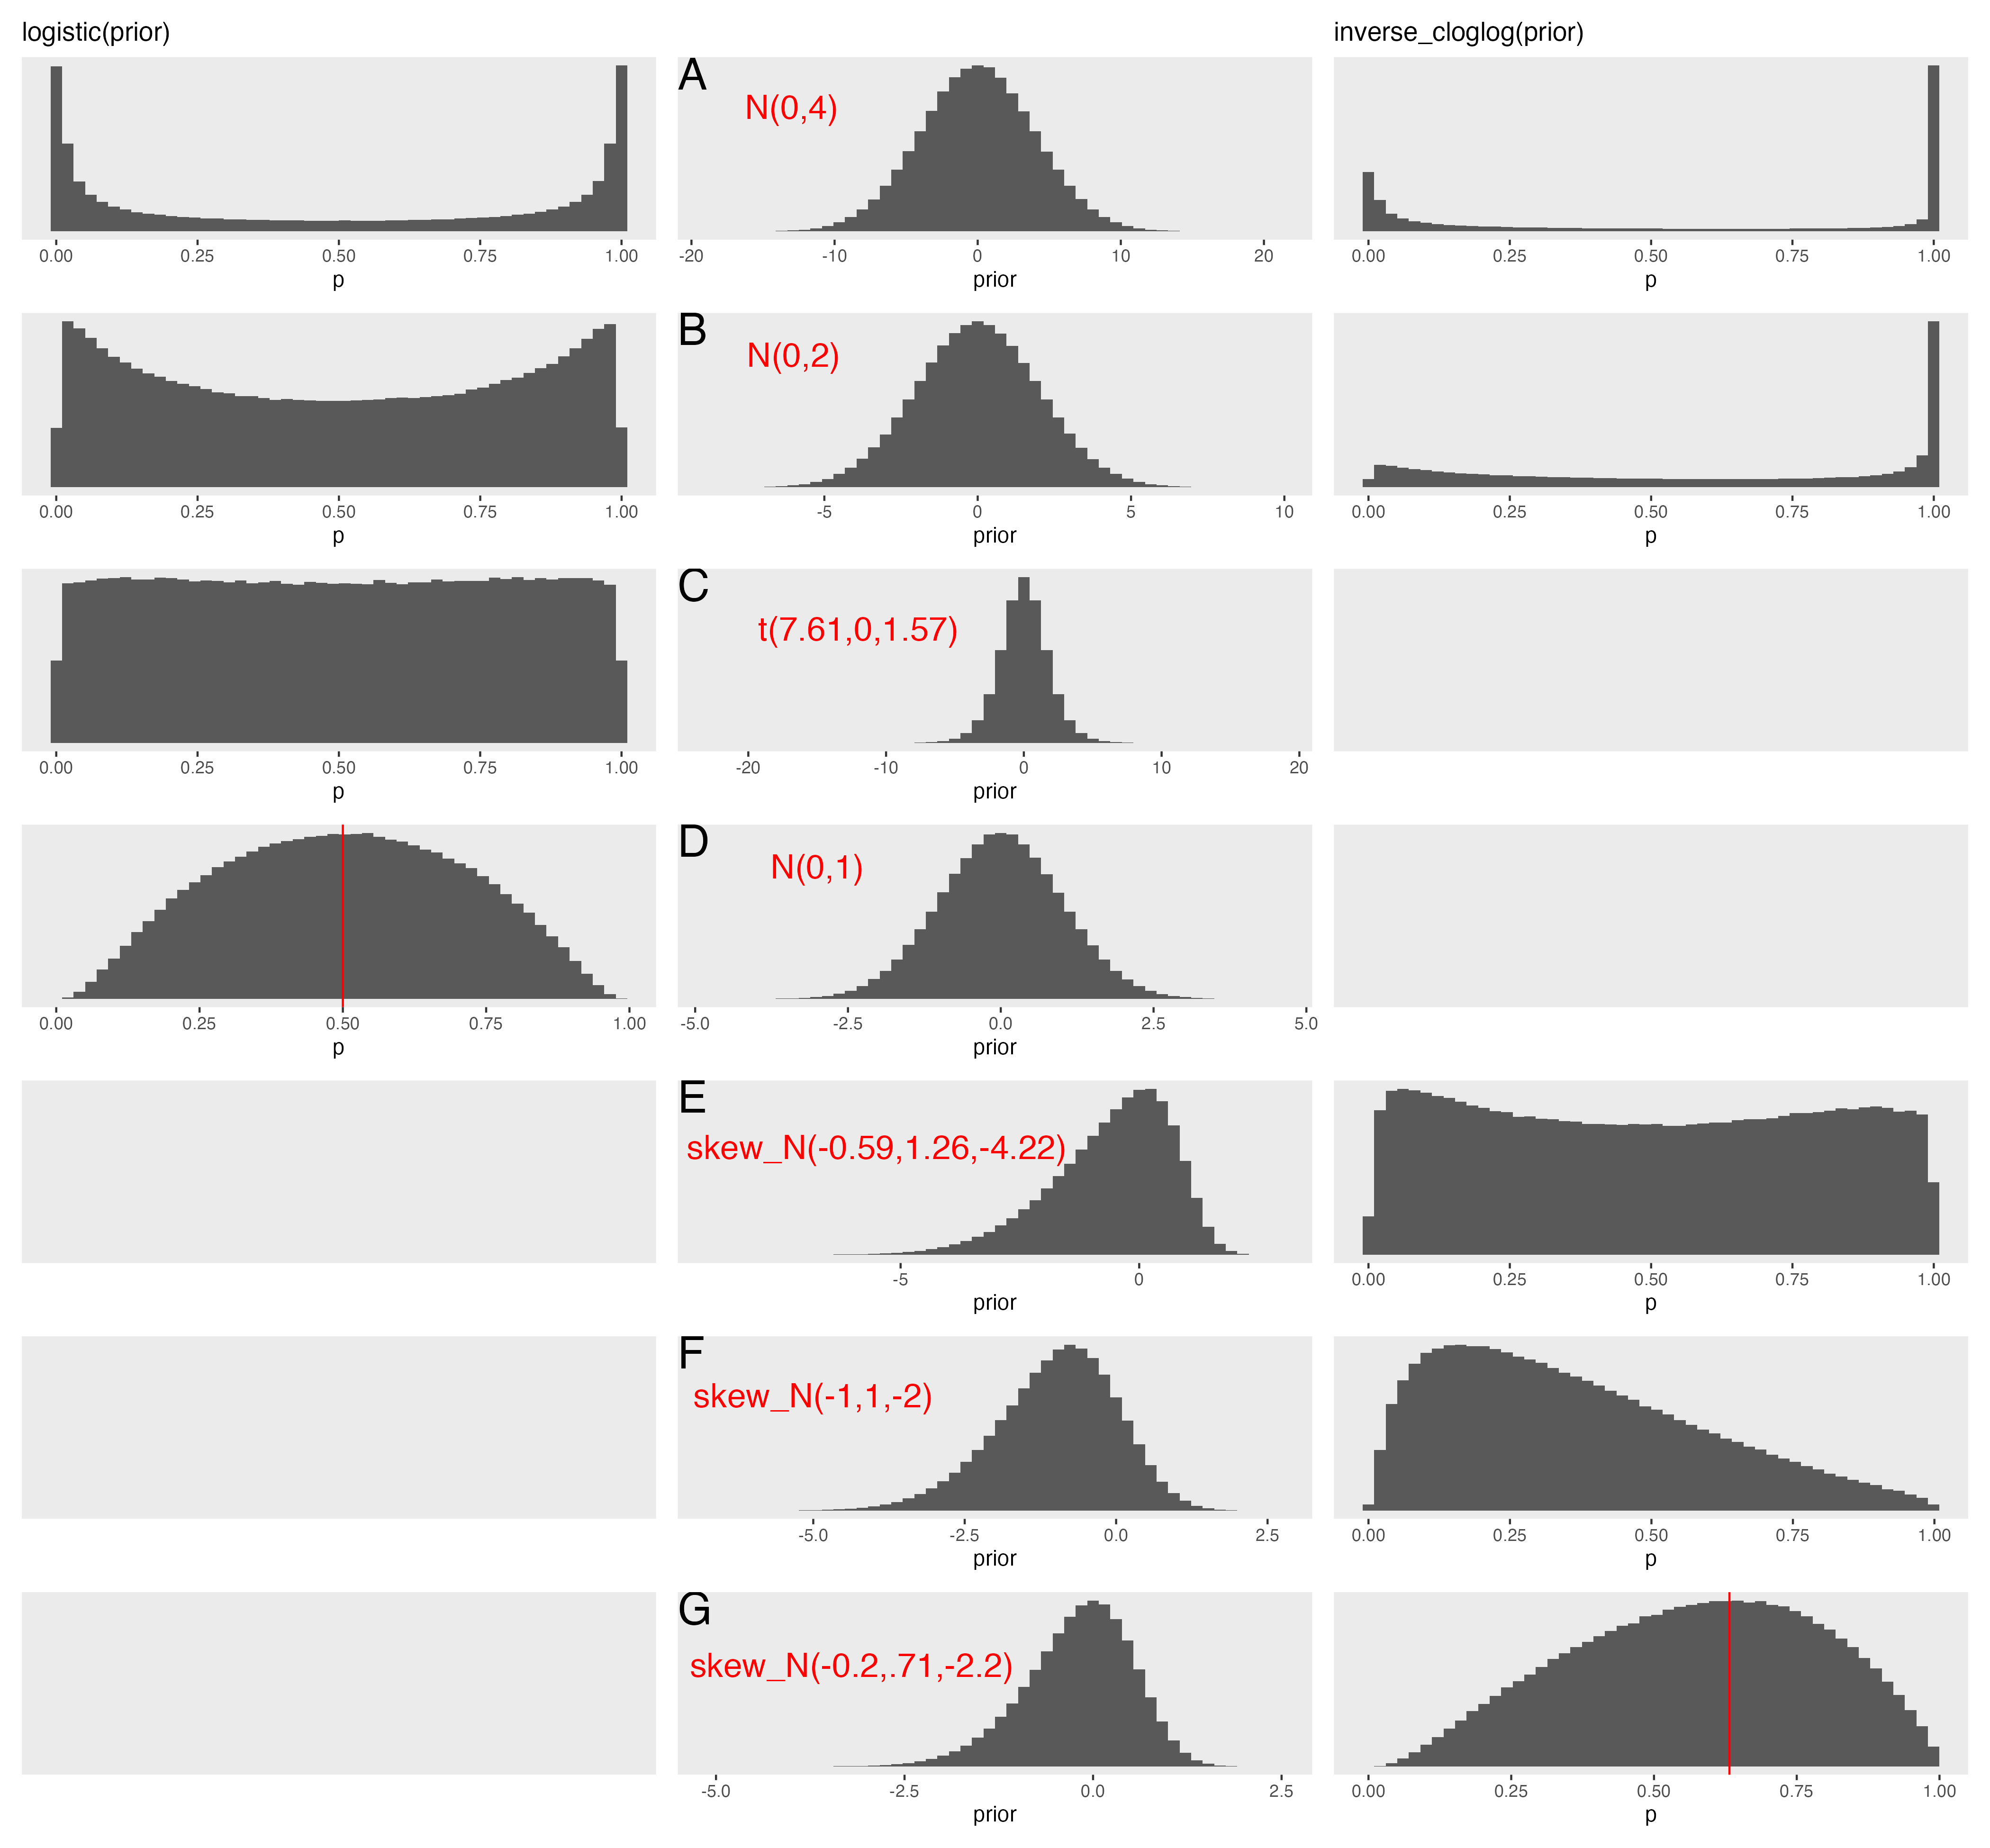
\includegraphics[width=0.8\linewidth,height=0.67\textheight,]{../Tutorial_2_Bayesian/figures/plot_of_priors} 

}

\caption{Prior distributions on the logit and/or cloglog scales (middle column), and their implications on the probability scale after applying the inverse-logit (or logistic) transformation (left column), and the inverse-cloglog transformation (right column).}\label{fig:plot-priors}
\end{figure}

To gain a sense of what prior \emph{cloglog} values would approximate a uniform distribution on the hazard probability scale, we followed Kurz's approach and simulated a large number of draws from the Uniform(0,1) distribution, converted them to the cloglog metric, and fitted a skew-normal model (due to the asymmetry of the cloglog link function). Row E shows that using a skew-normal distribution with a mean of -0.59, a standard deviation of 1.26, and a skewness of -4.22 as a prior on the cloglog scale, approximates a uniform distribution on the probability scale.
However, because hazard values below .5 are more likely in RT studies, using a skew-normal distribution with a mean of -1, a standard deviation of 1, and a skewness of -2 as a prior on the cloglog scale (row F), might be a good weakly informative prior for the intercept(s) in a cloglog-hazard model.
A skew-normal distribution with a mean of -0.2, a standard deviation of 0.71, and a skewness of -2.2 might be a good weakly informative prior for the non-intercept parameters in a cloglog-hazard model as it gently regularizes p towards .6321 (i.e., a zero effect on the cloglog scale).


\end{document}
